\documentclass{article}

\usepackage{graphicx,color,tabularx,amsmath,amssymb,fancyvrb,soul}
\usepackage{subcaption}
\usepackage{float}

\setlength{\parskip}{1em}

\title{CS310 Computer Science Project \\ Final Report \\ The Creation of an Android Application to Aid a Student's Revision of Edexcel GCSE Mathematics}
\author{Ryan O'Hara \\ u1702761}

\begin{document}

\maketitle

\newpage

\tableofcontents

\newpage

\section{Abstract}
\label{section:abstract}

%
%
%
%
%
%
%

\section{Introduction}
\label{section:introduction}

The introduction of this report aims to complete three tasks. The first task is to provide an understanding of the problem which this project wishes to solve. The second task is to explain the features required by this project to be deemed successful. These features were laid out in the project specification document[appendix 1] which was produced at the beginning of the project. Finally, this introduction aims to provide the reader with an understanding of the report structure, giving brief descriptions of each section in the report to explain their purpose.

\subsection{Problem Outline}

The difficulty of GCSE Mathematics recently increased due to a change in specification by Edexcel. This increase in difficulty was due to the UK Government's reform of the English and Mathematics GCSEs in November 2013[1]. The relevant section from the Department of Education's written statement to parliament is as such: "The new mathematics GCSE will demand deeper and broader mathematical understanding ...  The new mathematics GCSE will be more demanding". This demand for a deeper and broader mathematical understanding enforced a syllabus change for Edexcel's GCSE Mathematics qualification. This syllabus change started teaching in 2015, and examining in 2017[2]. \par

This increase in difficulty for GCSE mathematics is achieved through the introduction of more content into the specification. Because of this increase in content, a higher proportion of the academic year is dedicated to teaching, and students are left with less time to revise content for their exams in the classroom. This leaves students in the position of having to revise topics for their final examinations at home, typically without the support of a teacher or tutor. \par

95\% of American teenagers have access to a smartphone[3] a study from 2018 demonstrated. Also, a study conducted in 2017 stated "Recent statistics show that around 69\% of the total digital media time spent by Americans was taken up by mobile devices and 87\% of the total mobile time was spent in apps in December 2016"[4]. More students than ever before have access to smartphones, and they are spending the majority of their time on these smartphones in apps. More students have access to a smartphone than have access to a desktop or laptop computer as of 2017[3]. \par

Because of this increase in the availability of smartphones, students are now turning towards technology to aid with their learning and revision for their GCSE exams. This project aims to build a mobile application which can be used on the Android mobile operating system, which is the majority operating system (OS) for smartphone devices with a market share of 73\% between February 2019 and February 2020[5]. This allows the application to be available to the majority of students studying for GCSE mathematics. \par

This project aims to create an application which focusses on testing a student's current knowledge instead of teaching them new information. It is designed to be used alongside classroom teaching, or other less conventional teaching methods which aim to replace a classroom environment, such as Khan Academy. This application aims to focus on testing skills already gained by the user from a classroom like environment, and will emulate final year GCSE Mathematics questions to suitably prepare students for their end of year exams. \par

This application will have to provide users with the ability to practice skills gained from classroom learning. It must contain questions of GCSE exam standard so that students can effectively prepare for their exams using the application. It must also have the ability for users to input answers, and it must mark the answers and provide visual feedback to the user. A set of requirements created to complete these tasks is available below in the project specification subsection of this introduction. \par

\subsection{Project Specification}

This project aims to create an android application similar to the MyMaths homework functionality discussed in the background section of this report. This will enable student's to attempt exam questions in a specific topic in Edexcel GCSE Mathematics by inputting an answer. This answer will then be compared to the pre-calculated answer, and the student will get a visual response as to whether they have answered the question correctly or incorrectly. Where the student answered the question incorrectly, the correct answer will be displayed to the student so they can compare their answer with the correct one. \par

To achieve this task a set of requirements were detailed in this project's specification[x]. These requirements follow the MoSCoW method for specifying requirements. The MoSCoW method groups requirements into four classes, must, should, could, and won't. All of the must requirements are vital to the success of the project and so need to be completed by the end of the project. At the completion of all of the must requirements, a minimum viable product (MVP) is created and the product could be shipped. Should requirements are features which are not essential to the creation of a MVP but are features which are expected in the final product. Could requirements are features which are not expected in the final product, but if all other requirements are completed before the deadline, the could requirements will be implemented. Won't requirements are features which will not, under any circumstances, be present in the final product. \par

The requirements present in the project specification are as follows: \par

The Android application which will be created for this project must: 

\begin{enumerate}
	\item Have a start page with several clickable buttons
	\item Be able to run on Android devices with OS versions between Android 6 (Android Marshmallow) and Android 10
	\item Have a list of each module found in Edexcel's GCSE Mathematics Specification[6], with each module being a selectable button
	\item Generate revision questions where numerical values are generated by Java's inbuilt random number generator and are appropriate for the difficulty of the question
	\item Give the user the ability to input numerical answers to the revision questions generated (requires 4)
	\item Provide the user with feedback relating to whether their answer matches the correct answer for the question, and where the user’s answer is incorrect, display the correct answer. \par
	
	The Android application which will be created for this project should:
	\item Have a variety of testing difficulties, ranging from easy to hard for each module
	\item Have a way of tracking user progress over a number of days or tests per module (requires 5)
	\item Display model methods for working out the correct answer for a question where the user inputted an incorrect answer (requires 6) \\
	
	The Android application which will be created for this project could:
	\item Include resources similar to those which would be used in a classroom environment to teach the user about a topic
\end{enumerate}

Project success was also defined in the project specification. To be deemed successful, the final product produced by this project will have completed: 

\begin{itemize}
	\item all of the must requirements defined above
	\item at least one of the should requirements defined above
	\item any value of could requirements defined above
\end{itemize}

The target audience for the final product of this project is students sitting Edexcel GCSE Mathematics examinations. The average age of students sitting these exams are between 15 and 16 years old. Although, students as early as year 7 (age 11 - 12) begin learning content which is examinable in the GCSE Mathematics exam. The app will be primarily designed for 15-16 year olds, but needs to be accessible to students as young as 11. This means there are a group of non-functional requirements which were not outlined in the project specification but were created during development to ensure the target audience were taken into account. These non-functional requirements are shown below:

\begin{itemize}
	\item The language used in the application should be of a year 7 reading level
	\item The application should be simple and minimalistic as to not confuse new users
	\item An 11 year old who has not previously used the application but is familiar with smartphones should be able to use the application effectively with minimal prompting
\end{itemize}

These functional requirements enable anyone learning the content for the Edexcel GCSE Mathematics exams to be able to benefit from the application.

\subsection{Report Structure}

This report will start by running through the background to this project. The background section will outline the current landscape of the problem by exploring what has currently been achieved by other people in the field. It will be followed by an explanation of the software development methodology which was used throughout the development of this application. This methodology section will explain how the work was completed from a project management point of view, for example it will outline a typical development session. It will also explain any changes made to this methodology throughout this project. \par

Section \ref{section:design} outlines the design of the final product which will provide a high level overview of this application. This high level view will explain the control and data flows of the program, and any specific design choices which were made throughout the development of this project. Section \ref{section:implementation} discusses the specific implementation details of the project. For example, how the questions were created in the application. Testing will be discussed in section \ref{section:testing}. This will consist of outlining how testing was conducted, and the results of user testing. \par

The risk analysis conducted throughout this project will be explored in the risks section, which is section \ref{section:risks}. An outline of risks will be produced, followed by how each risk was handled, which will then be followed by the effect each risk had on the final application. Project management will be discussed in section \ref{section:projectManagement}. This section will explain several details of the project that cannot be understood by only viewing the source code for example the development schedule, or weekly meetings with key stakeholders. These details do not appear in the source code but have a great impact on the success of the project. The results section follows the project management section, where the requirements will be evaluated and the success of the project will be determined. \par

The conclusion will be section \ref{section:conclusion} which will summarise key findings in the report. This will be followed by the future work section which is extra work which could be conducted to improve this project, and turn it from a proof of concept into an application which would be able to be released onto the Google Play store. Section \ref{section:issues} will discuss the legal, social, ethical, and environmental issues associated with this project. \par

The final section in this report will be the references section, with a section number of \ref{section:references}. Harvard referencing style is adhered to throughout this report.\par

\section{Background}
\label{section:background}

There are three main GCSE Mathematics revision tools in use today that are recommended by schools. All of the main revision tools are explained in depth in their respective sections. Only one of the three main revision applications recommended by schools has a fully functional mobile application. There are also a number of other independent revision tools which are not actively recommended by schools, but are able to be downloaded and used on mobile devices. These tools are explored in the independent revision tools subsection. Finally, this section will discuss the research conducted at the beginning of this project into Android app development. \par

\subsection{MyMaths}

The first tool is MyMaths[7] which is a website which aims to enrich a student's classroom learning experience by supplementing material covered in the classroom. The main feature of MyMaths is the online homework feature. This feature enables teachers to set homework to their students. This homework covers a specific topic, for example Venn diagrams, and the students have to answer questions on this topic. Example homework questions on the topic of Venn diagrams can be viewed as figure \ref{figure:mymathsHomeworkQuestion1}.
\begin{figure}[H]
	\centering
	\frame{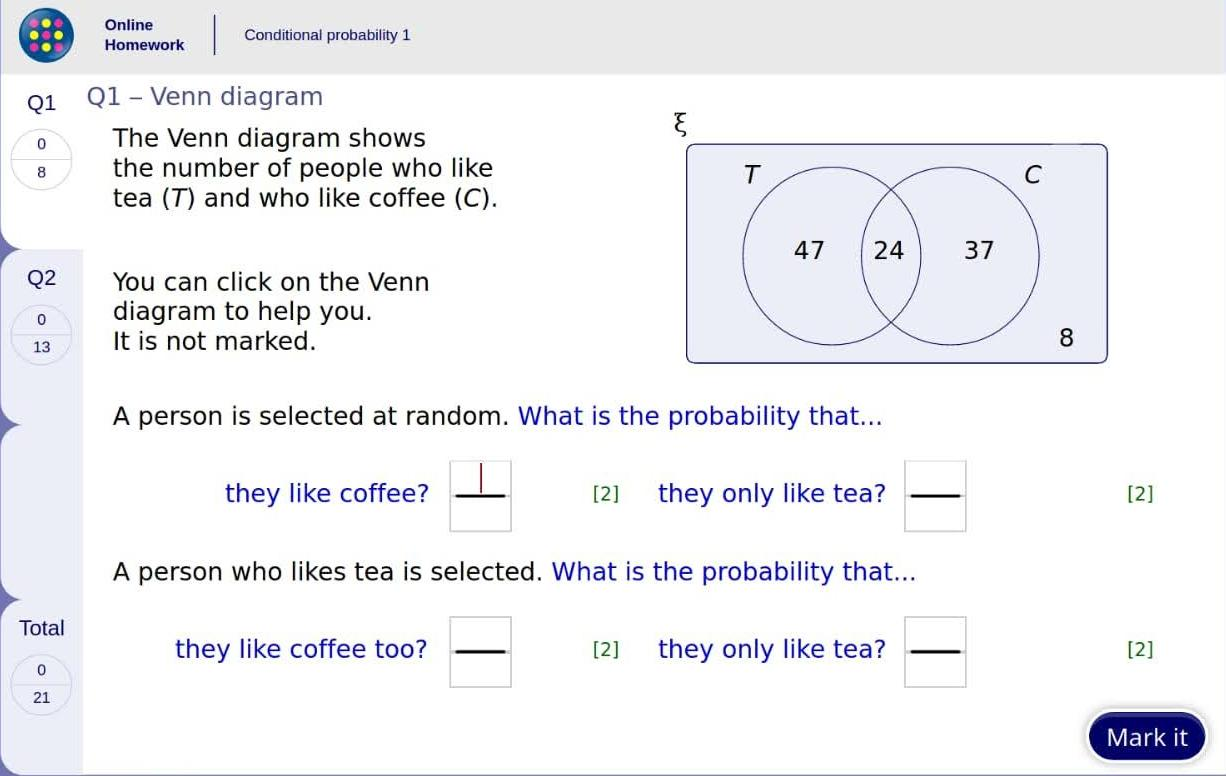
\includegraphics[width=0.9\linewidth]{./data/mymathsQuestion1.jpg}}
	\caption{Venn diagram homework questions.}
	\label{figure:mymathsHomeworkQuestion1}
\end{figure}
The student's scores are then calculated as a percentage and sent back to the teacher. \par

The values generated for every homework are unique each time a student attempts a homework. This prevents a student from memorizing a specific answer to pass the homework, also known as answer memorisation and is discussed in detail in the implementation section of the report. A teacher can also see the number of attempts that a student required to complete the homework, and their highest score. Providing teachers with the ability to see the number of attempts that a student needed to complete the homework for a particular topic highlights where a student is struggling and can enable one to one teaching to boost the student's knowledge in that particular topic. A student can also attempt a homework which has not been set by their teacher which allows any student to revise any topic in GCSE Mathematics on their own. \par

MyMaths also gives students the ability to take a lesson in any topic in GCSE Mathematics. These lessons walk through an example question in the topic, and then provide practice questions which are of a similar style to the homework questions. These questions are then marked, and where the student answers the question incorrectly, the correct answer is displayed next to the answer box. \par

MyMaths has an iOS and Android application for tablets, but not a specific application for smartphones[8]. This prevents students who own their own smartphones but do not have access to a tablet on a regular basis from utilising MyMaths as a revision tool. \par

\subsection{Khan Academy}

The second main GCSE Mathematics revision tool recommended by schools is Khan Academy[6] which is a non-profit organization which aims to "provide a free, world-class education for anyone, anywhere"[9]. Khan Academy's main function is to teach new information to people. It does this through the use of short, lecture like videos covering particular concepts. For example, there is a six minute video covering how to find a side of a triangle using the sine rule given two angles and another side[10]. These videos aim to replace classroom teaching for those who are unable to attend school. There is a video for every topic in GCSE Mathematics and so a student could exclusively use Khan Academy to learn the content for their exams. Khan Academy also has a testing feature, where for a certain topic four questions come up which the user has to answer one by one. This is, however, not available for all topics, and the user is limited to answering four questions at a time. \par

Khan Academy has mobile applications in both major app stores, the Apple app store[11] and the Google play store[12]. Their app runs on all major devices and has the same functionality as the website version of Khan Academy. Users can create an account for free which keeps track of their progress, although anyone can access videos for all topics available on their website and apps without one. This gives everyone with access to an internet connection the ability to watch any of the Khan Academy videos. \par

\subsection{Maths Watch}

Maths Watch[13] is an older tool which was used for teaching purposes in schools. It provides educational videos for students to learn from, as well as providing walk-throughs of past exam paper questions. It is designed to replace both classroom teaching, and as a homework tool. Maths Watch is a subscription service, which only schools can subscribe to. If a student's school is not subscribed to Maths Watch then a student cannot get access to it. \par

Maths Watch has two main methods for distributing their video content. The first method is through DVDs which are posted to the schools which buy them, and the students can then get these discs from the schools with all of the videos on them. The second method is through their online portal which provides the ability for paid users to stream video lessons. The Maths Watch service also states on the subscription page of their website[14] that they provide "A bank of 1000s of interactive exam-style questions for students' independent work with instant feedback". This is similar to MyMaths where a user can submit their answers and get feedback on whether they were correct, and if they were incorrect have the correct answer displayed. \par

The Maths Watch service is used by students all throughout the UK and is an incredibly valuable tool to aid their learning. Unfortunately, Maths Watch does not provide a mobile application on either of the major app stores (Apple iOS app store, or the Google Play store). As well as this, only schools can purchase Maths Watch, so if a students' school is not a Maths Watch partner, then the student cannot get access to Maths Watch. \par

\subsection{Independent Revision Tools}

There are several other mathematics revision applications on both major app stores, examples of which can be seen below as figure \ref{figure:appStoreApps}. These apps mostly focus on testing a user's knowledge using some form of revision questions. These questions are either limited to multiple choice answers, or questions which have the same values each time they appear. This leads to two problems: random guessing for the multiple choice questions, or answer memorization for the questions which do not change their values. This leads to these applications not being endorsed by schools. \par

\begin{figure}[H]
	\centering
	\begin{subfigure}{0.8\textwidth}
		\frame{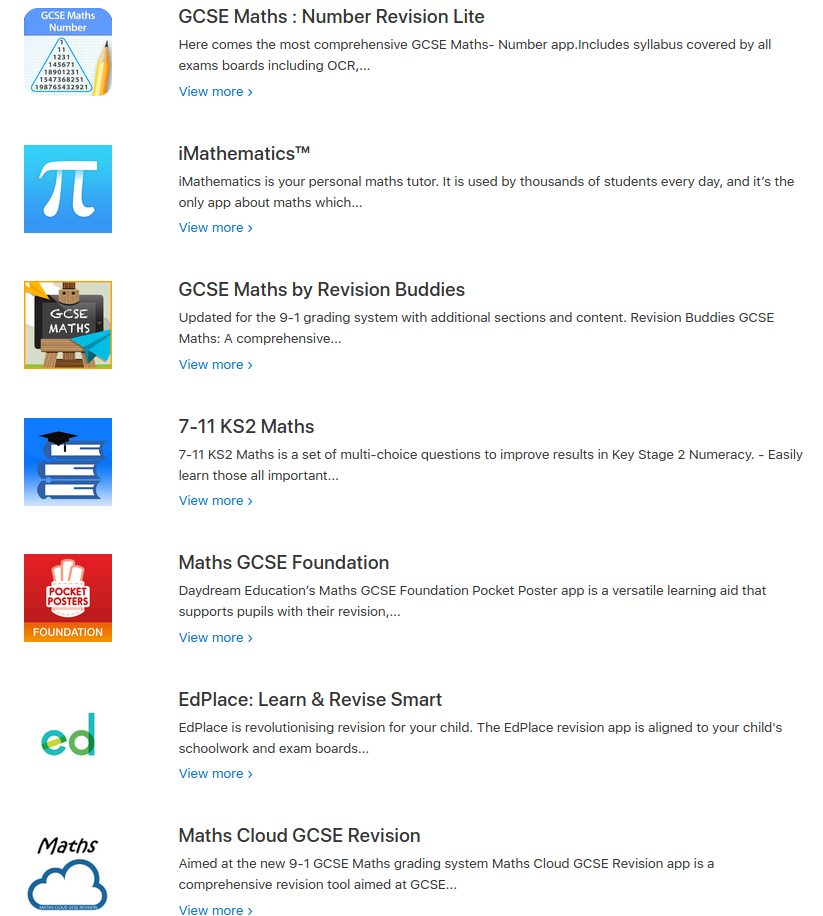
\includegraphics[width=0.9\linewidth]{./data/appleAppStoreApps.png}}
		\caption{Revision applications on Apple's app store}
	\end{subfigure}
	\hfill
	\begin{subfigure}{0.8\textwidth}
		\frame{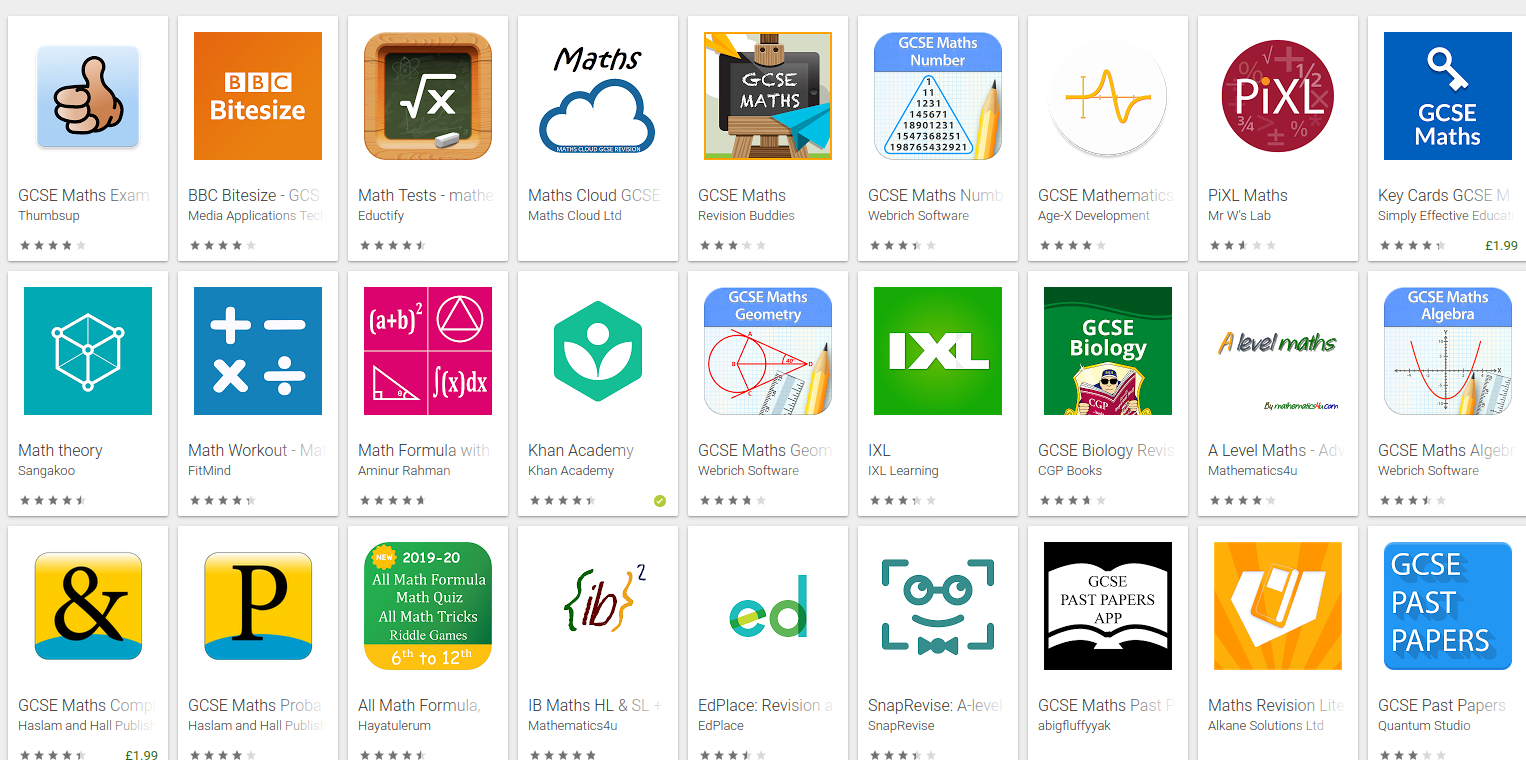
\includegraphics[width=0.9\linewidth]{./data/googlePlayStoreApps.png}}
		\caption{Revision applications on the Google Play store}
	\end{subfigure}
	\caption{Revision applications on both the Apple app store and the Google play store}
	\label{figure:appStoreApps}
\end{figure}

\subsection{App Development}

Research into Android application development consisted of: 

\begin{itemize}
	\item Working through Head First Android Development[15]
	\item Reading through the Android Documentation [16]
	\item Creating small Android apps available on github [17]
\end{itemize}

These tools were utilised in learning the basics of Android application development before any code was written for this project. The Android documentation helped with any programming issues within the code during the development of this application. 

\section{Methodology}
\label{section:methodology}

This section will explain how the work necessary for this project was completed. It will describe the process with which the final application was developed at a high level, and section \ref{section:implementation} will explain the lower level ideas with examples from the final application's source code. \par

The process with which work was completed within this project, often referred to as the methodology, changed throughout the duration of the project. The project specification stated that "This project will make use of the scrum software engineering methodology". The scrum methodology was not followed throughout the early stages of this project. Instead, a non-specific agile methodology was utilised, as each development cycle planned only the next requirement to be added as a feature. Each development cycle did not create user stories, or have a pre-defined length of between one and four weeks for development, which are both key features of the scrum methodology. \par

The non-specific agile methodology utilised for the early stages of this project consisted of four main steps. The first step was selecting the next requirement to be implemented into the program. Then any decisions that needed to be made concerning implementation details would be made and a small plan would also be created detailing these decisions. Finally, the code would be written for the requirement to the specification of the plan. Once the requirement was completed, there would be no review, and so development would move onto the next requirement. \par

Monitoring and controlling for all aspects of development was continuously conducted throughout this project. Midway through the project it was noticed that the methodology was not being followed as set out in the project specification. This problem is discussed in more detail later in the risks section of this report which is section number \ref{section:risks}. This deviation from the initial project plan was disruptive to the progress of the project, and so the methodology followed throughout development was changed midway through the project. It was still a non-specific agile methodology as no user stories were written, but each development (sprint) cycle consisted of one week, with specific time being dedicated each week to development. The other major change to the methodology was to include sprint reviews. These two changes meant that the methodology could be viewed as a variation on scrum which used the project's requirements instead of user stories. \par

The final methodology change for this project was implemented during the last month of development. It aimed to help with writing this report and continuing development in parallel as focussing on both was inefficient. Initially, all sections of the report were aimed to be written in parallel to decrease the amount of idle time in the writing process due to bottlenecks. For example, sections such as design required figures to be created which could not be worked on whilst also writing the report. Figures and images were created and added in at a later stage. This meant that if sections were worked on individually then there would be idle time whilst waiting for images to be created. To fix this issue multiple sections were worked on simultaneously when writing the report. This caused its own issues by increasing time spent context switching, which can be viewed as wasted time. Once the context switching increased above a specific boundary the decision was taken to switch the methodology for report writing from scrum to the Kanban development methodology. \par

This change in methodology manifested itself in two key ways. The first was using Trello[18] as a way of visualising workflow, which is a key principal in the Kanban software development methodology. A Kanban board was set up for writing the report, and can be seen as figure \ref{figure:trelloBoardOG}. 

\begin{figure}[H]
	\centering
	\frame{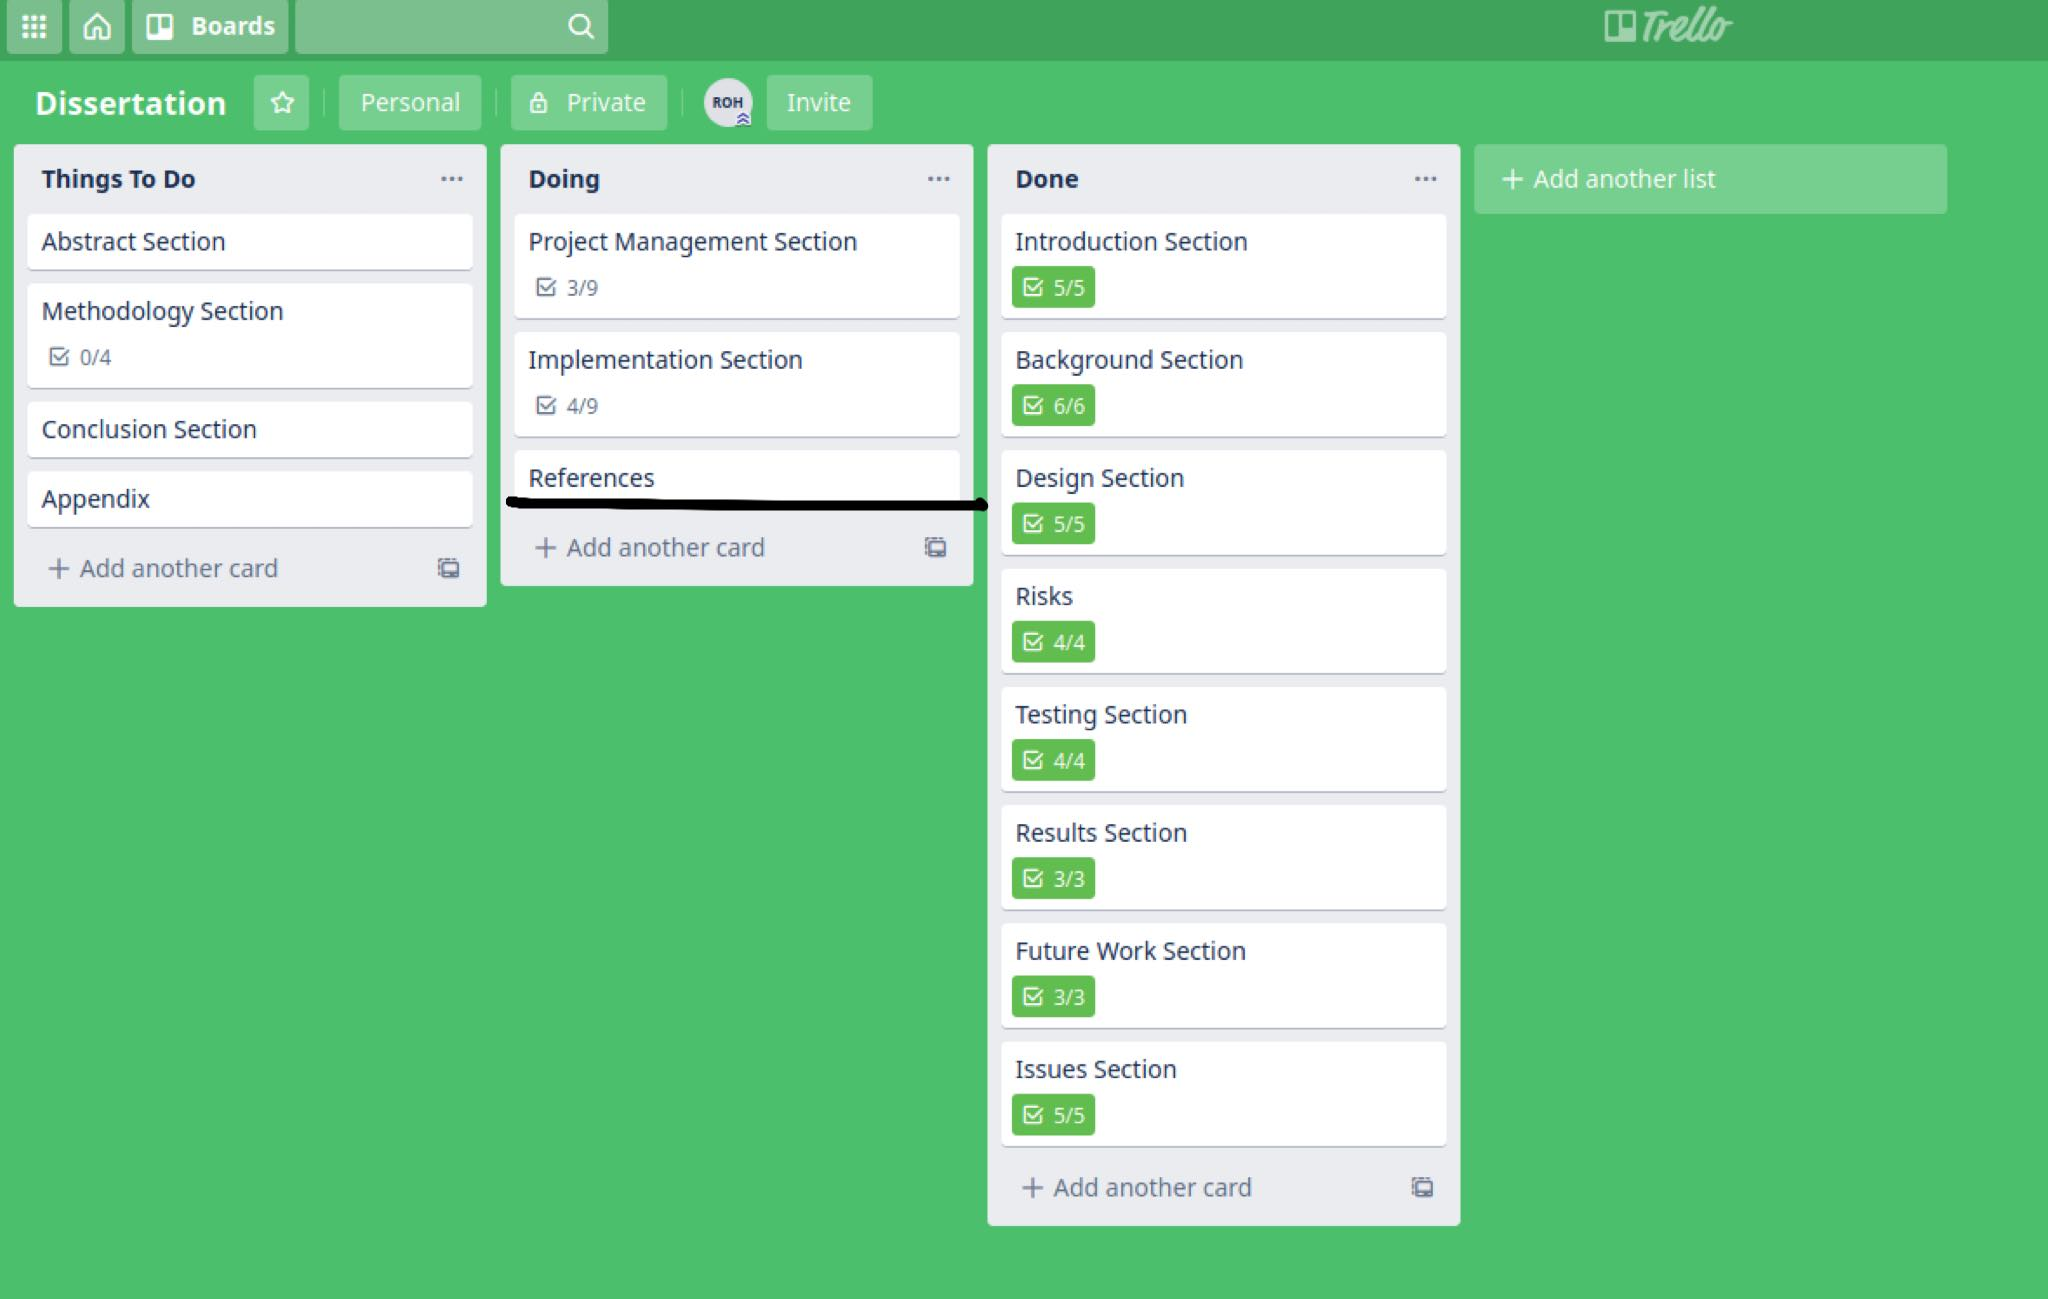
\includegraphics[width=0.9\linewidth]{./data/trelloCopy.jpg}}
	\caption{Trello board used as a to-do list for this report.}
	\label{figure:trelloBoardOG}
\end{figure}

This Trello board was created to effectively visualise the work that had to be completed for this report to be deemed finished. Work is pulled from the 'Things To Do' section into the 'Doing' section. Once the work is completed, it is moved into the 'Done' section. The second change to implement Kanban was the introduction of work in progress limits. Work in progress limits reduce the amount of time spent context switching by limiting the amount of tasks which can be worked on at any one point in time. There is one work in progress limit set in figure \ref{figure:trelloBoardOG} and is denoted by a black line under the 'References' card in the 'Doing' section. This work in progress limit decreased the amount of time spent context switching, and also narrowed the focus of each development session. Instead of having the choice between working on several sections of the report, the choice was between two sections of the report at any one time. This narrowed focus increased the productivity of the report writing, and also increased the quality of the text written. 

% Add a section about the implementation philosophy
%
%
%

\section{Design}
\label{section:design}

This section of the report will explain the visual design philosophy which was adhered to throughout development. It also aims to discuss the control and data flow of the final application. \par

This application had a target audience of school children between the ages of 11 and 16. This meant that any design would have to be simple and intuitive to prevent users from getting 'lost' within the application. The graphs for both the control and data flow for this application are acyclic as is shown by the two figures below, figures \ref{figure:applicationControlFlow} and \ref{figure:applicationDataFlow} respectively. Users can only follow certain paths, and will only end up in the same place by pressing the inbuilt backwards button in the Android operating system, so they cannot get confused about the layout of the application. Also, the number of pages was kept to a minimum for the application to function for the same reason. This minimalist design aims to prevent confusion by keeping the application simple to understand and use. \par

\subsection{Visual Design}

The visual design of this application is minimalist. Each activity only has the necessary information displayed on it, and where possible, only one item is displayed per activity. Below are a few examples of this minimalist design. Figure \ref{figure:applicationStartPage} is a screenshot of the application's start page taken from the physical Google Pixel 2 device.

\begin{figure}[H]
	\centering
	\frame{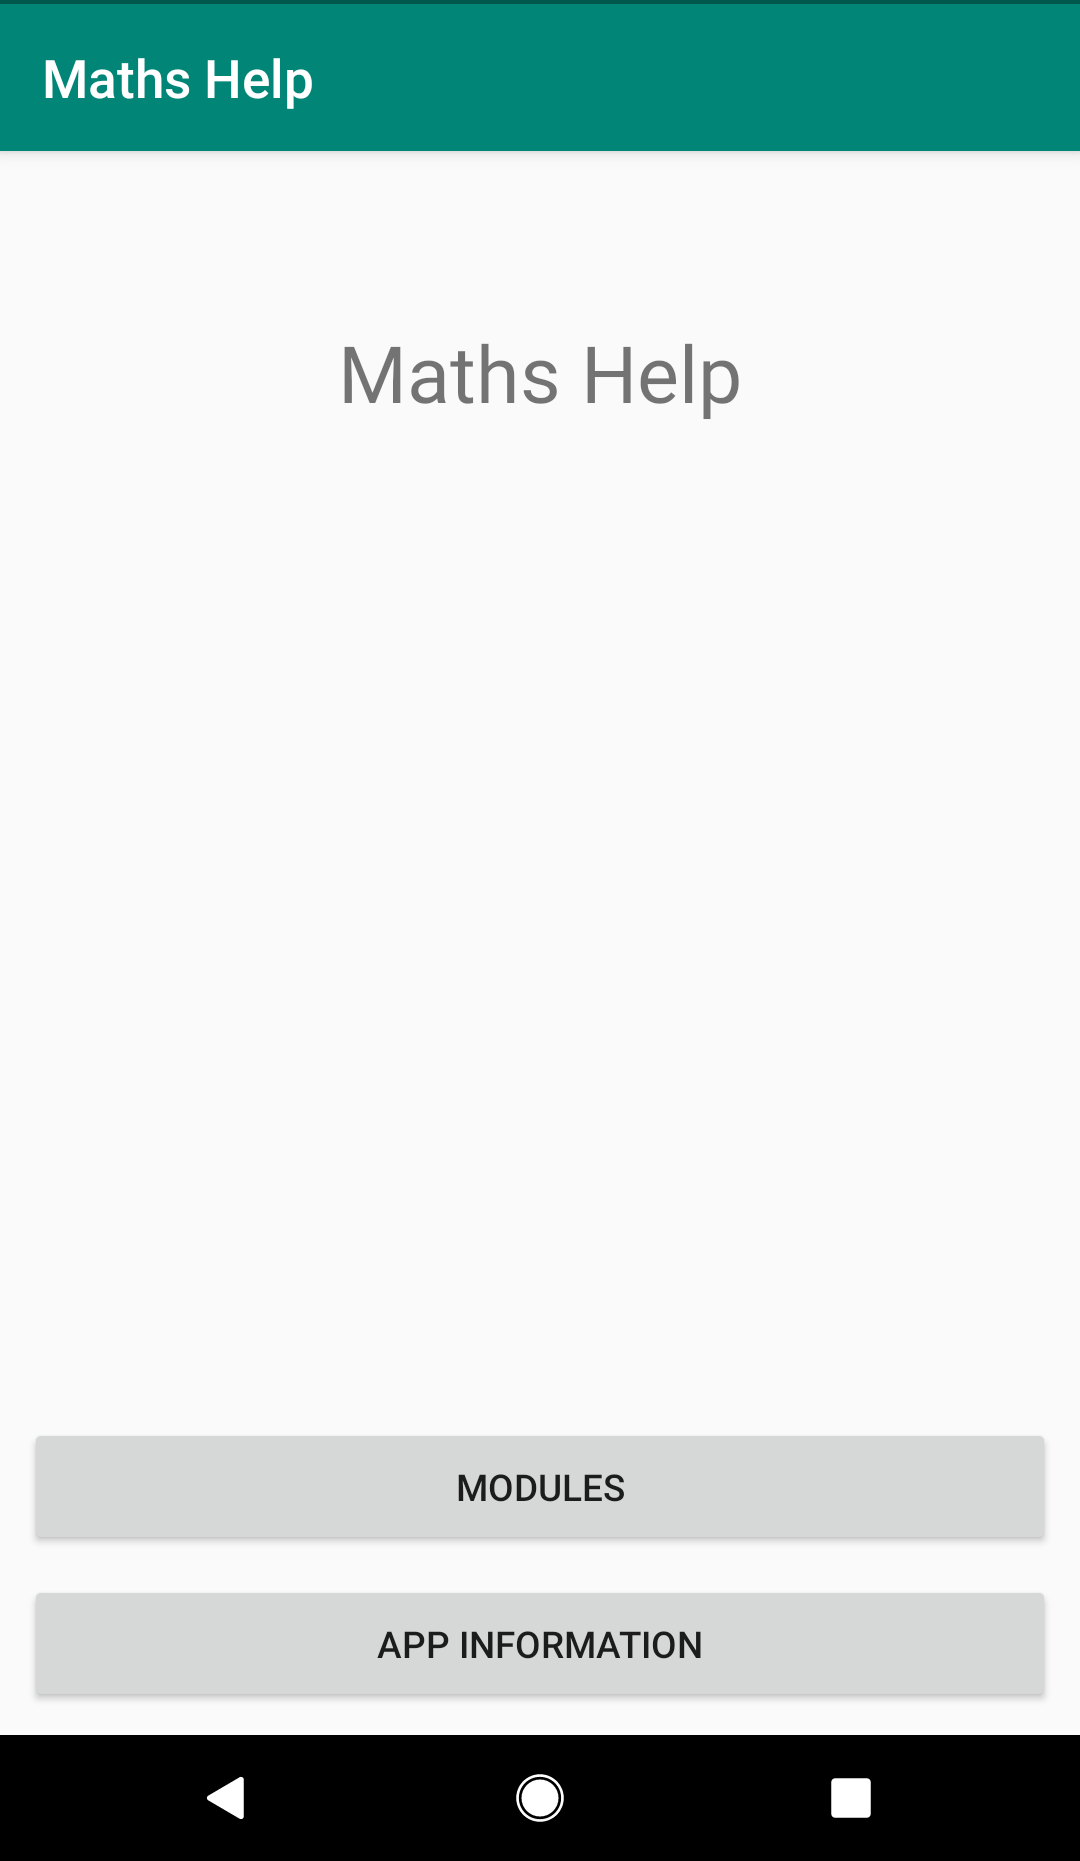
\includegraphics[width=0.5\linewidth]{./data/applicationStartPage.png}}
	\caption{Start page of the application screenshot from the physical Pixel 2 testing device.}
	\label{figure:applicationStartPage}
\end{figure}

This screen is made up of the least amount of distinct elements that is possible. As it is the start screen of the application, and is the first thing a new user will see when using the application for the first time, it has to have the application name displayed which is the "Maths Help" text at the top of the screen. The bottom of the screen is dominated by two buttons, one which starts the modules activity (the modules button), and one which starts the information activity (the app information button). There is nothing else visible on the page, and this is the least amount of elements with which to follow the control and data flow graphs displayed below. \par

An example of the activities displaying list fragments is the modules activity screen. This is displayed below as figure \ref{figure:applicationModulesPage}, also taken from the physical Pixel 2 testing device. 

\begin{figure}[H]
	\centering
	\frame{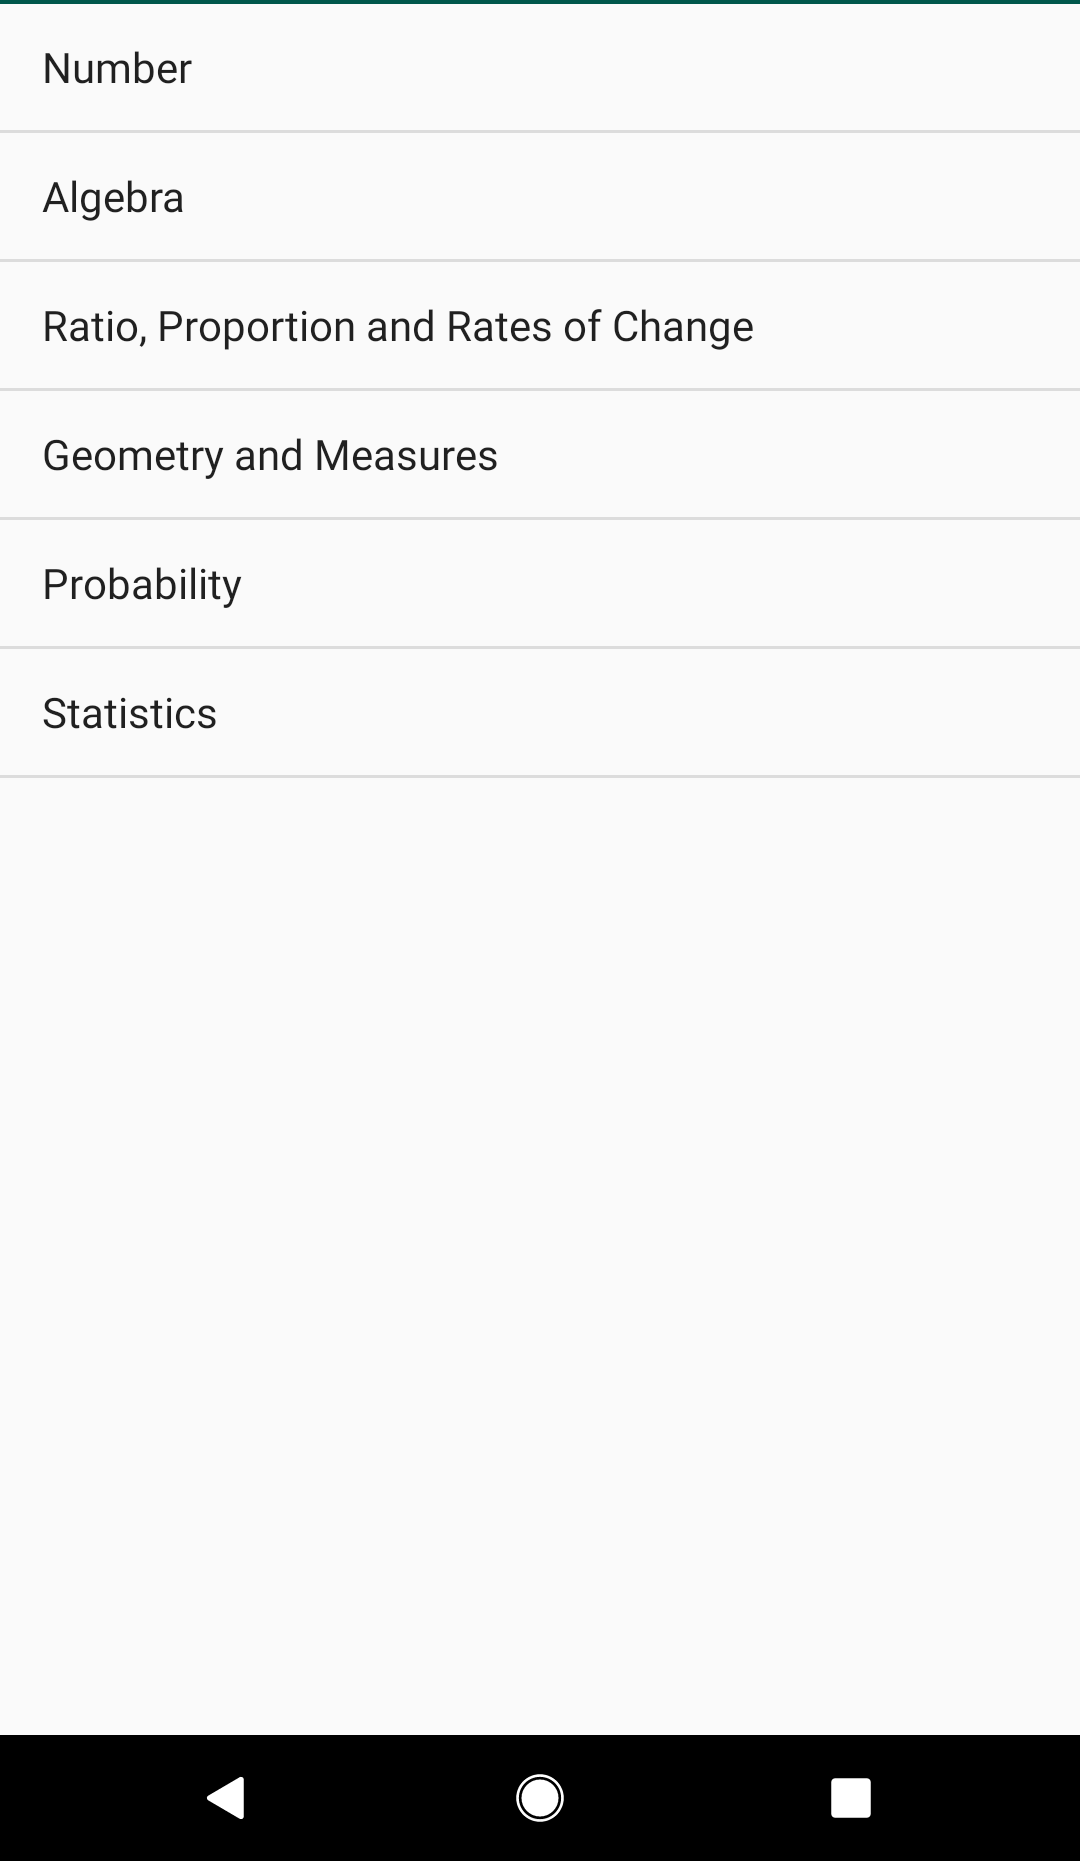
\includegraphics[width=0.5\linewidth]{./data/applicationModulesPage.png}}
	\caption{The modules activity page.}
	\label{figure:applicationModulesPage}
\end{figure}

This screen is empty except for the selections that a user can choose. This basic design ensures that only what is essential for the application to function is included on each screen. All of the screens which contain a list could have included an explanation at the top of the screen informing the user to select one of the options. This was not included as each user involved in black box testing intuitively understood how the lists functioned. It was deemed that an explanation would clutter the screen, users could see it as condescending, and it could negatively impact the user experience. \par

The question display activity also obeys the minimalist design of this application, only containing what is essential for the question to be answered. It can be seen as figure \ref{figure:applicationQuestionPage}, which is a photo of the screen taken from the physical Pixel 2 testing device.

\begin{figure}[H]
	\centering
	\frame{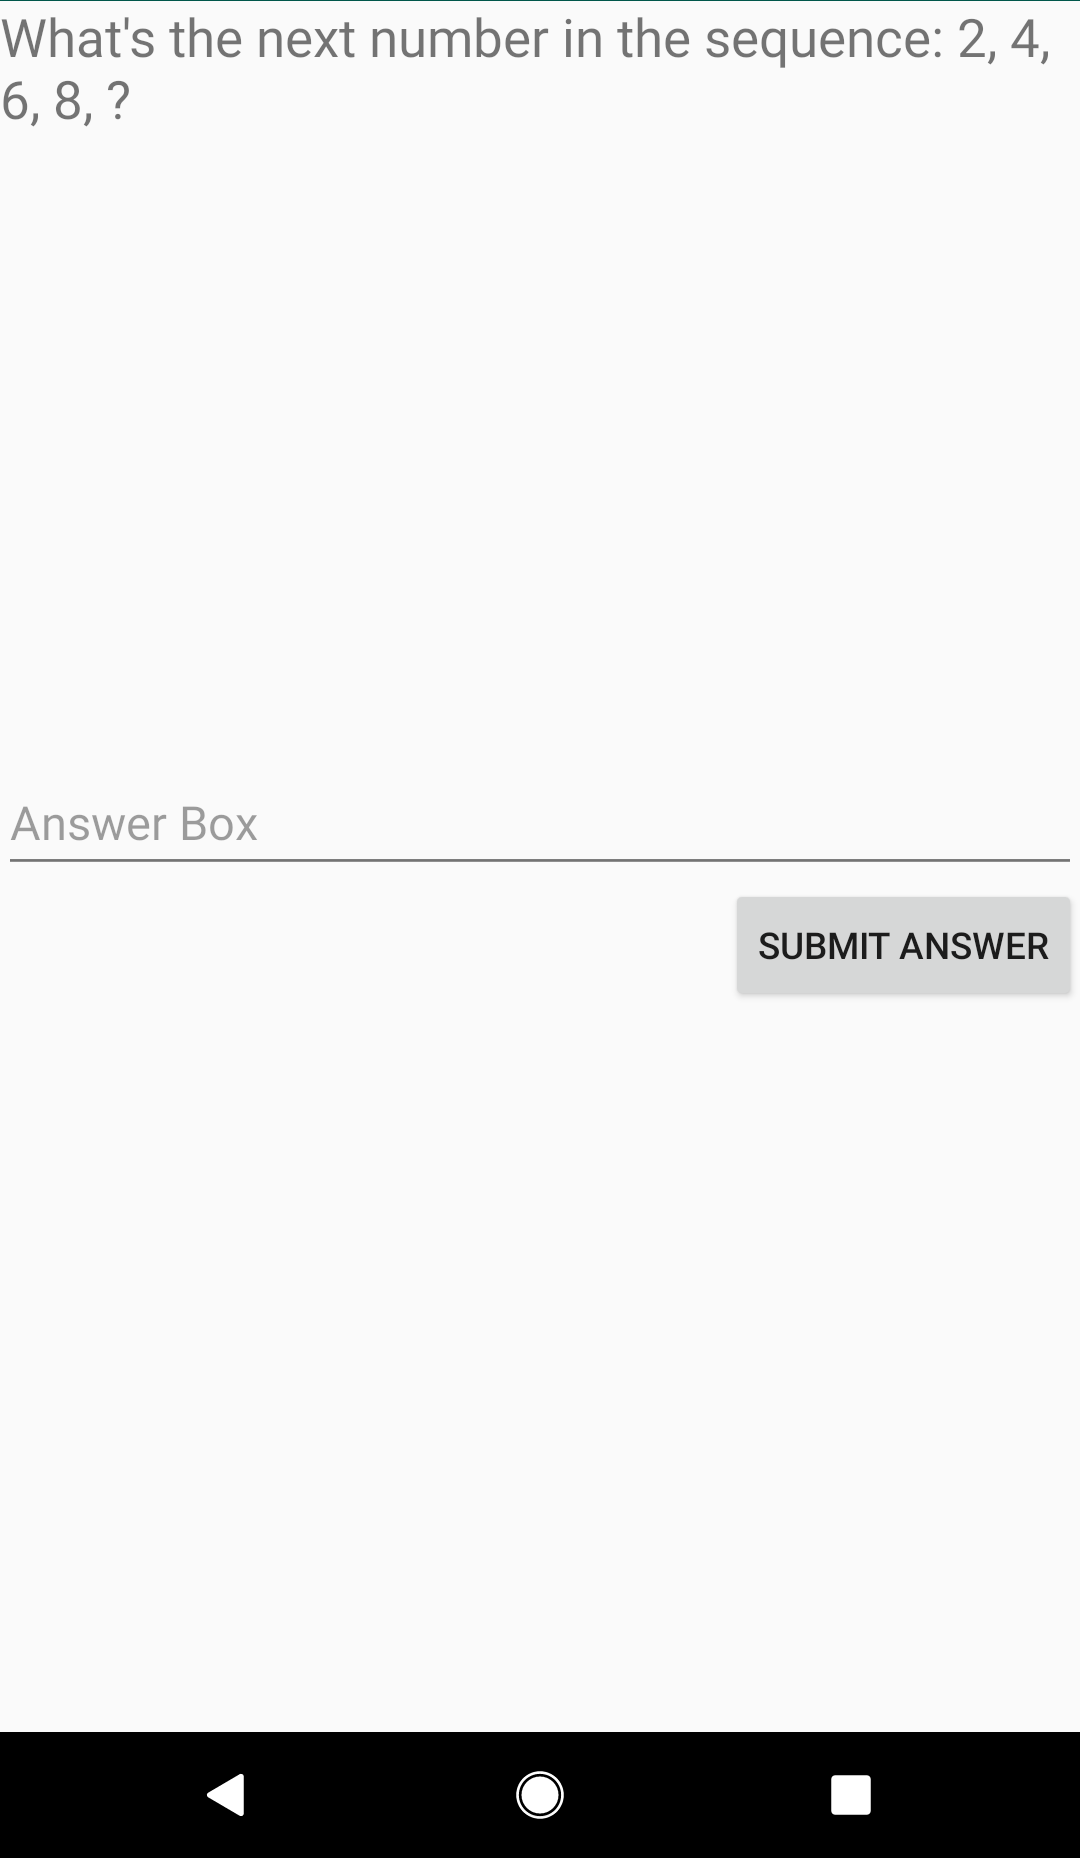
\includegraphics[width=0.5\linewidth]{./data/applicationQuestionPage.png}}
	\caption{The question display page.}
	\label{figure:applicationQuestionPage}
\end{figure}

This activity consists of the question text, an answer box for the user to input text, and a submit button. For questions in which an image is required the image appears between the question text and the answer box. A minimalist design is followed throughout the application, to include only what is necessary on each activity as to not over complicate the application. \par

\subsection{Control Flow}

Figure \ref{figure:applicationControlFlow} is a graph for the control flow of the application. Each edge is bidirectional, the user can move forward by interacting with the application, and backwards by hitting the Android operating system back button. The user interacts with the application in one of three ways, either by pressing a button on their screen, selecting an element from a list in front of them, or entering text into a text field. \par

\begin{figure}[H]
	\centering
	\frame{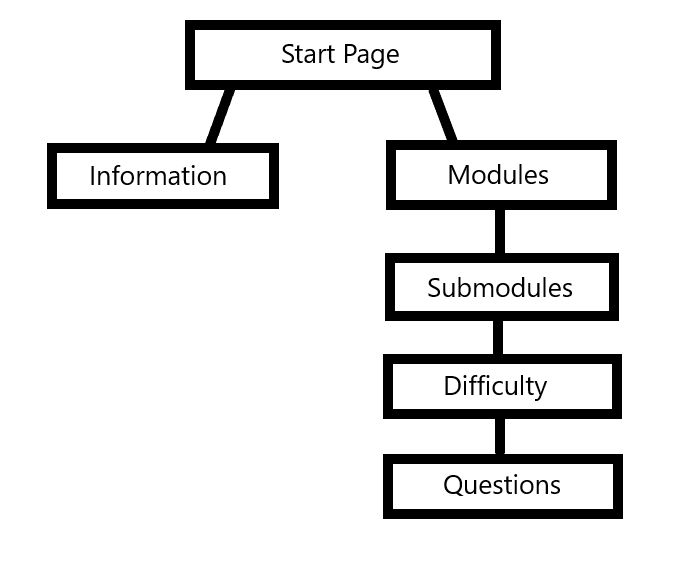
\includegraphics[width=0.6\linewidth]{./data/applicationControlFlow.png}}
	\caption{The control flow of the application.}
	\label{figure:applicationControlFlow}
\end{figure}

The only choice in direction in this application is at the start page where a user could select between the information page for the application and the modules list. Each node in this graph represents an Android activity. An Android activity is the application equivalent to a webpage on a website. Activities are viewed as one screen in an application[19] and are intended to complete one specific task. If another task needs completing then the application should call another activity. Activities can contain fragments which can be thought of as "a modular section of an activity ... (sort of like a 'sub activity' that you can reuse in different activities)"[20]. The modules, submodules, and difficulty nodes in the control flow graph displayed above are activities which only contain list fragments. The list fragment class is a subclass of the fragment class but is adapted to display a list of items, and implement a listener which will act when the user clicks on an element in the list. In the example of the modules node in the control flow graph, the list fragment displays all six modules which are examined in Edexcel GCSE mathematics. When the user clicks a specific module, the modules activity collects the information of the module selected from the list fragment, and starts the submodules activity with the information of the selected module passed to it as an input. The submodules activity then displays a list fragment containing the submodules for the module selected by the user. \par

The control flow for this application is minimalist. It only includes pages which are absolutely necessary. The graph for the control flow of the application is intentionally acyclic. Without any loops there is only two ways in which a user can end up at a certain page, they can go forward from the root node, or they can go backwards from a leaf node. This is simple, and should not confuse users, as they can only follow linear paths within the application. If a user ends up at a page that they have encountered before then they must have pressed the Android back button. \par

\subsection{Data Flow}

Figure \ref{figure:applicationDataFlow} is a graph of the flow of data throughout the application. When an activity starts another activity, it can pass information to it. This enables a single directional information flow throughout the application. That is why the diagram displayed as figure \ref{figure:applicationDataFlow} is a directed graph. The direction of the data is denoted by an arrow, the side of the edge without the arrow is the activity sending the data, and the side of the edge with an arrow is the activity receiving the data. 

\begin{figure}[H]
	\centering
	\frame{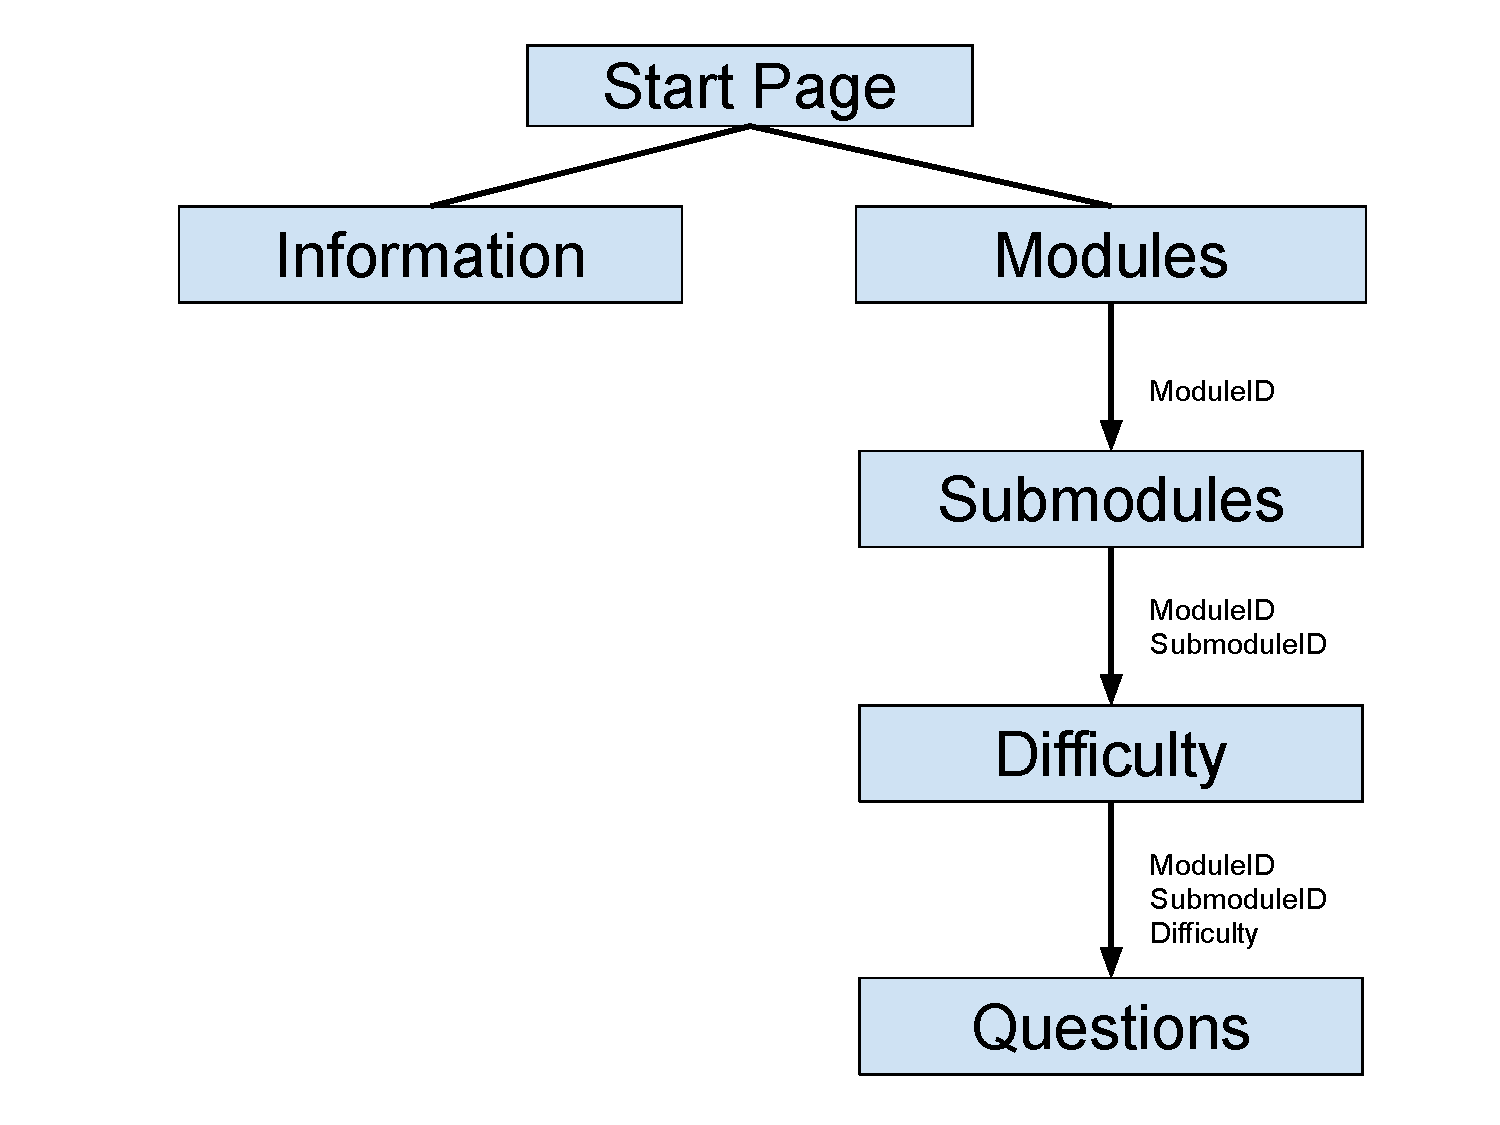
\includegraphics[width=0.9\linewidth]{./data/applicationDataFlow.pdf}}
	\caption{Diagram representing how data flows through the application.}
	\label{figure:applicationDataFlow}
\end{figure}

The data flow in this graph follows the minimalist design of this application. Data moves along a path in only one direction. A user can go back to a previous activity by using the inbuilt back button in Android. By doing this, the information selected further up the graph (closer to the root node) is preserved, but the information gathered along the edge which the application is now traversing is lost. This allows a user to utilise the back button to change the difficulty of the questions that they are answering whilst keeping the module and submodule information preserved. This enables simple use, where a user does not need to reselect all information to change one specific piece of data. \par

Information is passed along the modules path until it gets to the questions activity. The questions activity then uses all of the information to select the questions that it will display. \par

\section{Implementation}
\label{section:implementation}

This section will discuss how the project was created, providing examples from the source code where appropriate. It will explain in depth some key features of Android development and how they have been applied to this project, and will also justify key decisions made throughout the development process. 

\subsection{Fragments}

Android activities have been explained earlier in the design section of this report. A fragment is very similar to an activity, and has a very similar life cycle. Fragments can be viewed as a modular section of an activity. One activity can contain multiple fragments, and the same fragment can be used in many activities. A fragment is designed to be used when a developer wishes to run the same code in multiple activities, and is a way of preventing developers from rewriting code. As fragments can be added to activities in the same way a text box is, it is quick and simple to reuse code by utilising fragments. \par

Visual elements of the application are stored as XML data and then rendered on the device. Each activity has its own XML data to tell the device how it should be rendered. This allows each activity to have its own unique layout created to achieve the task assigned to that activity. Fragments also have their own XML data which enables a unique layout to suit their specific goals, and they can have their own code. Fragments, however, have to be attached to a parent activity. This allows fragments to act similarly to how an activity would in a given situation. \par

In this project fragments have been used in the place of activities for lists. This allows for different layouts to be created for the different sizes of devices, for example the application could look different on tablets than it does on smartphones. Although, changing the visual design of the application depending on the size of the device it is running on is currently unused in this application as it is straightforward, it could allow for different layouts between different devices when the application gets more complex. It could also allow lists to be displayed next to each other on larger devices. For example, the submodules list could appear alongside the modules list when a module is selected. This only works if there is enough space available on the screen to display two lists next to each other. \par

As previously stated in this report, this project used fragments, specifically the listFragment class, as opposed to activities, specifically the listActivity class, to control the modules, submodules, and difficulties lists. There are examples, however, of where activities have been used instead of fragments. This is due to the reuse ability of the code. For example, the questions page of the application is currently an activity where it could have been an activity composed of fragments. The displayQuestion activity could be modified to utilise several fragments instead of being an activity. Displaying an image could be implemented as a fragment which displays the image, and then the fragment could be included in the displayQuestion activity. All of the other segments of the displayQuestion screen could have been implemented as a fragment. This, however, was decided against. For consistency, the questions are displayed identically on all devices as to ensure a good user experience. Since the code was only going to be used once, it was written as an activity. \par

\subsection{Questions}

Three key decisions were made in regards to how questions were implemented in the application with varying consequences. \par

The first key decision that was made regarding implementing questions into the application involved selecting the questions to be included within the app. It was essential that the questions included in this application were of GCSE standard so that students could effectively revise for their exams. The decision was made to pull the questions included within the application from past Edexcel GCSE Mathematics papers. Examination of the new Edexcel specification began in the summer of 2017 and was conducted twice an academic year in November and June. This project was conducted between the fall of 2019 and the summer of 2020. This allowed for six different sets of past papers for the current Edexcel GCSE Mathematics specification at the beginning of this project. Each of these sets included three foundation tier papers and three higher tier papers. Each question paper included between 20 and 30 questions, which provided a lower bound of 720 past paper questions provided by Edexcel. This allowed for a large pool of questions to be added into the application, spread across all of the modules and submodules tested within Edexcel GCSE Mathematics. \par

The process of adding new questions into the application began with labelling each question from a past paper with the module and submodule that it belonged to. This information, combined with the difficulty of the paper that it was included in, meant that the path that a user would have to take through the application to get to the question could be mapped. It also highlighted the amount of questions which were similar to the one in the exam paper which are already present within the application. This gave the ability to balance the questions, ensuring that each module and submodule had the same amount, which meant that each topic could be revised thoroughly. \par

The second key decision that was made regarding implementing questions into the application was their storage medium. There were three key methods of storing the questions for this application. They were: hard-coding the questions into the application, reading the questions from a JSON file on the user's device, or selecting specific questions from a SQLite database as SQLite is included by default in Android. For this project the questions were hard-coded into the application. The two other implementation methods are explained in detail in section \ref{section:futureWork}. The decision to hard-code the questions into the application was made due to the methodology used to develop this software. As discussed in section \ref{section:methodology} when developing the application an MVP was rapidly achieved, with that MVP then being built on to add more features. Because of this, when the question feature was initially being implemented into the application only one question was included. Once that question was successfully tested other questions were added into the application. The fastest way to implement a single question into the application was to hard-code it into a class. Once the initial question was implemented further questions were added in batches of four. \par

The third key decision regarding question implementation was how to hard-code them into the application. A questions class was created which included all of the information that a question would need within the application. A question object would be created every time a question was required for the application and would include all of the information about the question so that it could be displayed and answered. A screenshot of the question class can be seen below as figure \ref{figure:questionClass}. 

\begin{figure}[H]
	\centering
	\frame{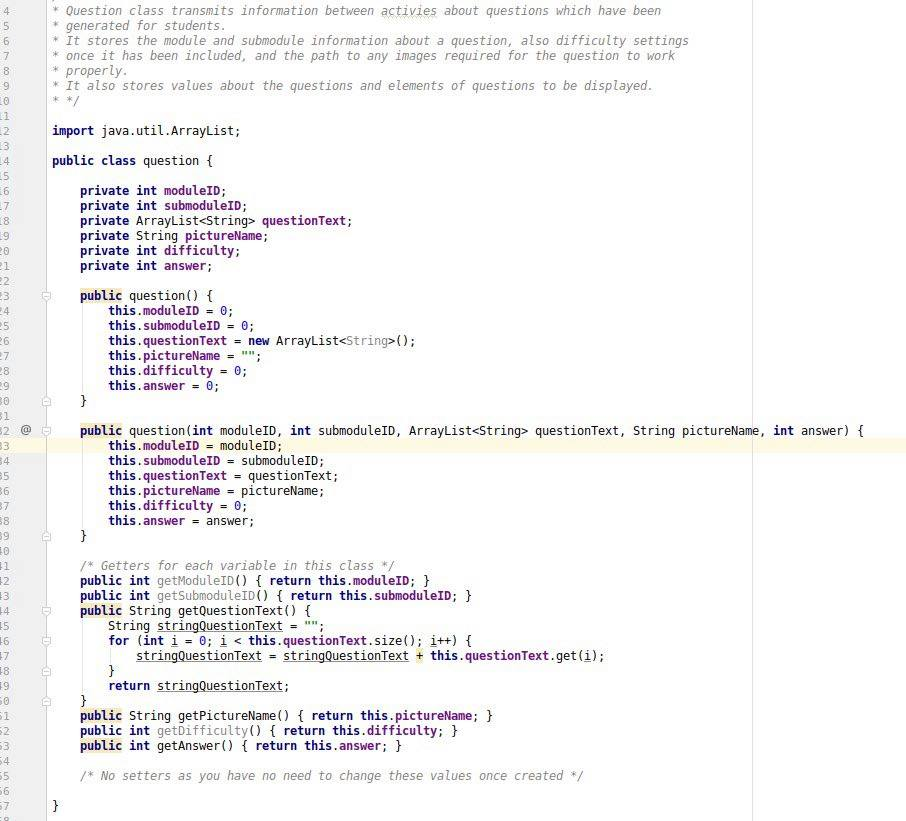
\includegraphics[width=0.9\linewidth]{./data/questionClass.jpg}}
	\caption{Source code for the question class.}
	\label{figure:questionClass}
\end{figure}

This class stores both the moduleID and submoduleID for a question. It also includes an array list which stores data in a Java string class. This array list contains the question text data, which is then showed to the user by the displayQuestion activity. The getQuestionText() method iterates through the array list accessing each individual element and concatenating it into a string to return to the displayQuestion activity. This data is stored in an array list instead of as a string for convenience. It is convenient because it enables the question text to be split on the numerical values which are used within the questions. The final array list will be in the form "text, (number, text)*" where this form is viewed as a regular expression and a "," indicates a new element is to be created within the array list. This enables the ability to put numerical values into the question text but also provides access these values if needed. \par

The string pictureName included in the question class in figure \ref{figure:questionClass} is the file name of the image which will be displayed along with the question text. Currently, only one image can be displayed, although this could be extended to multiple images by storing the file path of the images in an array list which would then be iterated through. If this variable is set to the string "None" then the image view is hidden from the screen, and no image is displayed. The question difficulty is also stored in this class as a numerical value being either zero or one. A zero stored in this field indicates that the question is a foundation tier question, whereas a one value being stored indicates that the question is from a higher tier paper. \par

The question's answer is also stored in the question class. All question answers have been rounded to integer precision and all questions include information stating that the user's answer should be rounded to the closest whole number value. On top of the text being included in each question users are prevented from entering non-integer values into the text box as they will be marked as incorrect. Currently, no questions which require text based answers are included in the application, although they could be implemented. These kinds of questions would be included in multiple choice format, with radio buttons displaying prospective answers, and users would select the answer that they thought was correct. The application would then send the answer as a value between zero and n, where n is the number of prospective answers being displayed, to be marked. The background of the correct answer could then be displayed as green to indicate that it is the correct answer, and the background of the incorrect answers can be changed to red. \par

Where a numerical value is used in a question it has been produced in one of two ways. It has either been produced using the Java random method, or it is calculated from other numerical values which have been randomly produced for the specific question. This ensures that numerical values for questions are values which have not been seen before by a user, or are not repeated often. This aims to prevent answer memorisation. Answer memorisation is where a user enters an incorrect answer for specific question values, and then remembers the correct answer which gets displayed, and so next time a student is presented with the same question with the same values, they input the answer which they remember from the last time they attempted the question and it is marked as correct. This makes it look like the student has learned the method for answering the question, when in reality they have just memorised the answer for those specific values. This is why when a value is used in a question it is generated using the Java random method over a specific range of values. This allows the student to see new values often whilst attempting a specific question, but it also allows the answers to be appropriate for the difficulty level of the question. \par

For a specific submodule several questions are generated. When a user selects a specific submodule, one of the questions associated with that submodule is produced to be answered. These questions currently have an equal probability of being selected, but the frequency of each question appearing could be adjusted. \par

Figure \ref{figure:testQuestionGeneration} is an extract from the source code of the application. It is from the testQuestionGeneration.java file. This section of source code generates the test questions and answers, and returns a question class with all of the relevant information in it. 

\begin{figure}[H]
	\centering
	\frame{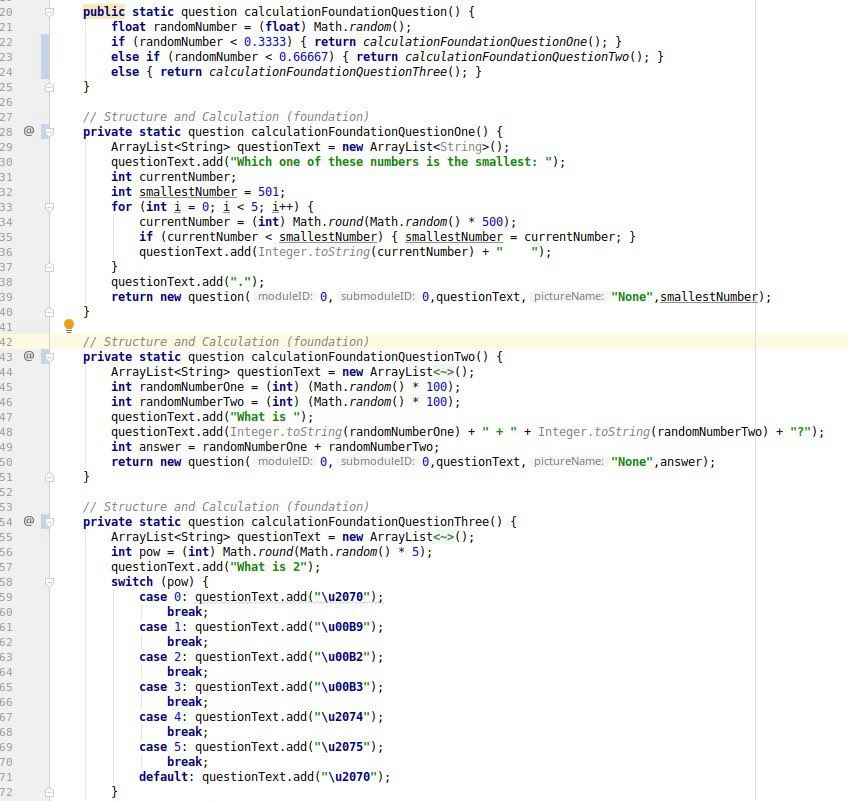
\includegraphics[width=0.9\linewidth]{./data/testQuestionGeneration.jpg}}
	\caption{Source code for the random question generation}
	\label{figure:testQuestionGeneration}
\end{figure}

The testQuestionGeneration class, which is displayed above as figure \ref{figure:testQuestionGeneration}, is a factory class which returns random questions given module and submodule details. The calculationFoundationQuestion() method is called when the user selects the number module followed by the structures and calculation submodule. It returns one of three questions written for the structures and calculation submodule, selected using Java's random number generator. The random question is generated by the appropriate private method in the factory class. For example, calculationFoundationQuestionOne() is a private method which generates a question object with the appropriate information. This method generates five random numbers between 0 and 500, and the user is asked to input the smallest number of the five. This question object is then returned to the calculationFoundationQuestion() method which then returns the question object to the displayQuestion activity allowing the question to be shown to the user. Each submodule has their equivalent of the calculationFoundationQuestion() method in this factory class. \par

\subsection{Control and Data Flow}

A decision was made when it came to the control flow of the application. As is stated earlier in this report, a list fragment is used to display both the modules and submodules lists, as well as the difficulty list. It was decided that the moduleID selected from the modules list fragment was to be passed to one submodules list fragment that would collect the list to display based on the moduleID that it received. Instead, six list fragments could have been created, one for each module, and when a moduleID was selected from the modules activity, it could call one of these six list fragments depending on the moduleID that the user had selected. This would have greatly increased the complexity of the application from a development perspective, although would not have changed the user experience of this application. Figure \ref{figure:controlFlowComparisons} below shows the control flow diagram for this application, as well as the complex control flow diagram which splits the submodules activity into six individual submodule activities, each representing a separate module.

\begin{figure}[H]
	\centering
	\begin{subfigure}{0.45\textwidth}
		\frame{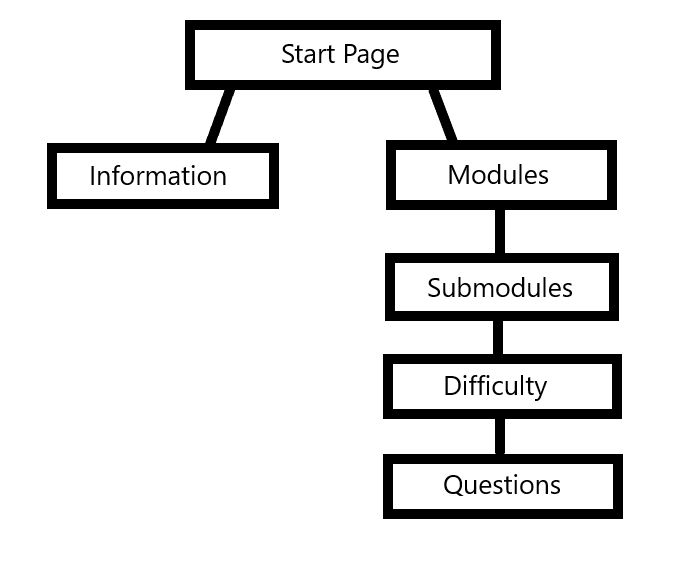
\includegraphics[width=0.9\linewidth]{./data/applicationControlFlow.png}}
		\caption{A diagram of the control flow of the final application.}
		\label{subfigure:applicationControlFlow}
	\end{subfigure}
	\hfill
	\begin{subfigure}{0.45\textwidth}
		\frame{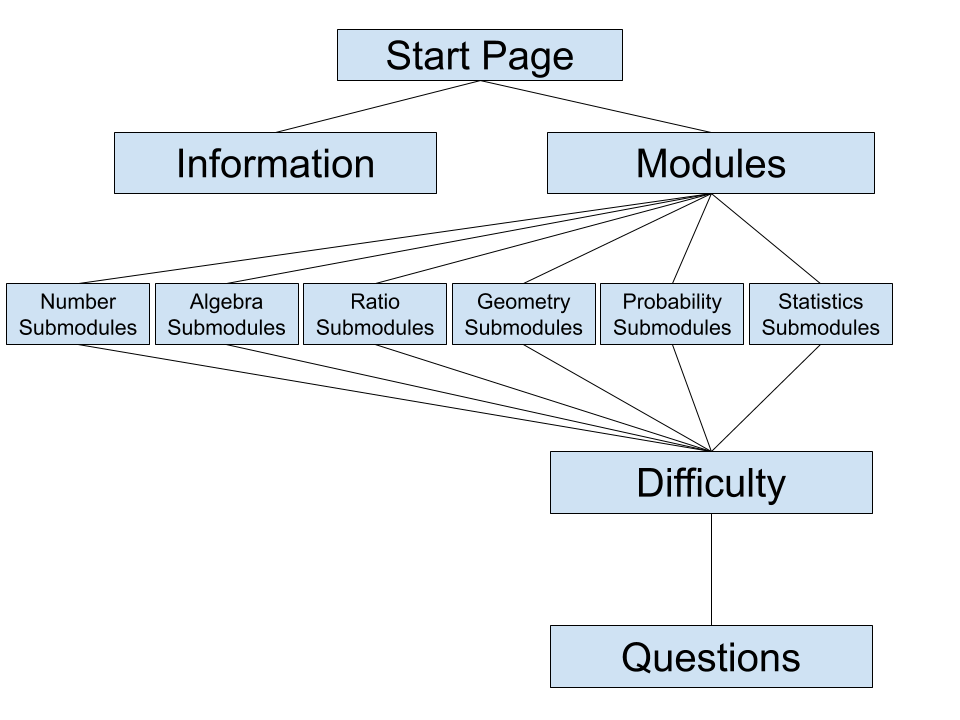
\includegraphics[width=0.9\linewidth]{./data/adaptedControlFlow.png}}
		\caption{A diagram of the control flow for the hypothetical complex application.}
		\label{subfigure:adaptedControlFlow}
	\end{subfigure}
	\caption{A comparison between the two choices in control flow for the application.}
	\label{figure:controlFlowComparisons}
\end{figure}

The second image, sub-figure \ref{subfigure:adaptedControlFlow}, has almost twice as many activities as sub-figure \ref{subfigure:applicationControlFlow}, and as such would have increased the time spent developing the application without providing benefit to users. This is why the decision was made to have only one activity which would fetch the appropriate list of submodules depending on the module selected by the user. This would also make adding a module or submodule simple, as it would just require adding the name of the new module or submodule to the appropriate array. If the other method of fetching a list of submodules was implemented, as sub-figure \ref{subfigure:adaptedControlFlow} displays, then adding another module or submodule would involve changing the control flow of the application by adding extra activities. This would have increased the complexity of the control flow of the application without adding benefit to the user, and goes directly against the minimalist design principle used for this application. 


\section{Testing}
\label{section:testing}

This section of the report will describe the general testing methodology conducted throughout this project after explaining why the testing methodology was changed. It will then explain the two kinds of user testing conducted for this application. 

The project specification[x] stated that this project would implement test driven development. The progress report[x] described that test driven development would not be used as the testing methodology for this project, and that user testing would be used throughout the project in its place. \par

The decision to change from test driven development to user testing was made because this project creates a tangible final product in the form of an Android application. An android application is judged by users for unquantifiable reasons, such as the "feel", or "ease of use" of the application. This can only be tested by a person using the application, and since this determines how satisfied a user is with the product, testing for the unquantifiable qualities of the application was prioritised over writing testing code. Writing unit tests for an android application was deemed to be an inefficient use of time, as this time could be spent improving the user experience of the application. \par

All application testing was conducted on a physical Google Pixel 2 smartphone, as well as at least one emulated virtual device. The emulation software used is built into the Android Studio IDE. It is called Android Virtual Device and [21]"... provides almost all of the capabilities of a real Android device". The emulator provides an environment to test the application on a variety of smartphones and tablets with different capabilities to ensure that the application works on a wide range of systems running the Android OS. The application was tested on three virtual devices: 

\begin{itemize}
	\item HTC Nexus One (Smartphone)
	\item HTC Nexus 10 (Tablet)
	\item Google Pixel 3 (Smartphone)
\end{itemize}

These testing devices give a good variety in the Android operating system, between both tablet and smartphone, and old and new. These devices were chosen because if the application works well on all four, the physical Google Pixel 2 phone as well as the three virtual devices, then the application was likely to work on most hardware running the Android OS. \par

Two types of user testing were conducted throughout this project, white box testing and black box testing. \par 

\subsection{White Box Testing}

White box testing is when someone who has access to the source code of the application, in this case the application's developer, is given access to the app and asked to complete a specific task. It was conducted after each sprint cycle, and consisted of the developer downloading the application onto their physical pixel 2 testing device as well as the range of virtual devices mentioned above, and then testing that the application compiled and ran without errors. Other small tests were also conducted when integrating new features. An example of this feature test would consist of the developer creating expected states of the application given specific inputs, and then following the input sequence on all four testing devices to ensure that the application finished in the expected state for each device. Visual tests were also conducted, where an activity's layout was drawn on paper, and then loaded on each of the testing devices. The layout on the testing devices was compared with the layout drawn on paper, and if the two layouts were identical then the activity passed. This testing method was used to find visual errors in the application and was conducted when changes were made to the XML of an activity. \par

\subsection{Black Box Testing}

Black box testing is when someone who has no access to the source code of the application is given access to the app and asked to complete a specific task. It was conducted using users outside of the development team. These users were not shown the source code for the application, and this testing was conducted primarily on the physical Pixel 2 testing device. The user would be provided with the application and their use of it would be observed. Before any testing was conducted verbal consent was gained from the user for testing the application through observing their use case. If it was the first time the user had seen the application then they were asked to try to use it as if they had just downloaded it from their normal app store. Whereas, if a user was familiar with the application then they were asked to complete a task which utilised a new feature. They could also be asked to compare visual styles with an image of both the current and previous styles, although the user was not made aware of which style was the current application style and which was the previous application style. Where there was a change in a feature that the user had used before, they were not notified of the change, and how they dealt with the change was noted. \par

Black box testing was conducted after every major feature was added to the application, with the results being used to improve the feature. Users of different mathematical ability were asked to test the application, from colleagues who use mathematics every day in their fields of study, to those who last encountered it when they took their GCSEs. \par

\section{Risks}
\label{section:risks}

This section will discuss some of the risks associated with this project. The risks will be outlined, which will explain the causes of the risks and the effect they would have had on the project. Once the risk has been outlined then the discussion will be around risk handling. All risks were handled in one of four ways. The risks were either: avoided, transferred, mitigated, or accepted. Where a risk was avoided, the cause of the risk was eliminated from the project. A transferred risk was one where the risk was handled by a third party, an example from outside of this project would be the case of authentication. If single sign on was used then the risk of password leakage is transferred to the third party responsible for the authentication. If a risk was mitigated then the effects of the risks were reduced by either reducing the probability of the risk occurring, or by reducing the impact that the risk had on the project. An accepted risk was one where no action was taken before the risk occurred, and when it did occur it was promptly dealt with without a large impact on the project. Finally, the outcome of the risk is discussed. \par

\subsection{Scope Creep}

Scope creep occurs when the scope of the project slowly increases over time. This occurs due to one of two reasons, either a customer keeps on changing their description of the final product, or the project manager adds unnecessary features to the project. As there is no customer directly involved in the development of this project the only way scope creep can occur is if the project manager adds to the initial feature set. \par

Scope creep can be incredibly damaging to a project in one of two ways. The first way is if the project does not have a predefined deadline and features continue to be added throughout development then the project may never be completed. If the project is evaluated for resources at the beginning of the project and scope creep occurs, then there may not be enough resources to complete the project. The second way that scope creep can be detrimental to a project is if the project has a deadline, then adding new features means less time is spent on key features for the project. When a resource is constrained scope creep can waste the resource and leave less of that resource for key features. \par

Scope creep was handled in this project by outlining the key features necessary for this application at the beginning. These key features are the requirements written in the project specification. Also, defining project success in the project specification helped to handle scope creep. The requirements outlined the key features which should have been developed throughout this project and the definition of success provided a baseline for the necessary features of the application. The requirements were written using the MoSCoW method to ensure that key requirements had a higher priority for development, and so were added into the application first. This mitigated scope creep by lowering the probability that it occurred. The requirements with a higher priority were completed first and created the MVP for the project. Once this MVP was created, the should requirements started to be implemented into the application. This prioritisation meant that any new features that the project manager wanted to add had to become could requirements, and so would have been added into the application after all key features. \par

This project did not suffer from scope creep. The requirements were a key reason for this as they dictated what was completed in a specific sprint cycle. As work was only conducted on the requirements with the highest priority there was no ability for features which were not included in the initial requirements to be worked on, and so no time was wasted. \par

\subsection{Personal Issues}

Due to the development team consisting of only one person who was irreplaceable to the project any personal issues on behalf of that individual could have affected the project. Personal issues could include a high workload, family issues, or a global pandemic. Any issues which would prevent the individual from working on the project due to reasons outside of the development cycle were classed as personal issues. \par

Personal issues are issues which cannot be prevented as they are unpredictable and can have varying affects on a project. This meant that personal issues had to be accepted. As personal issues were a group of issues which were unrelated to the project, but still affected it, it was possible to mitigate or transfer these individual issues. For example, if a personal issue is that the only member of the development team were to fall ill and be unable to work for two weeks, then it would have been mitigated with a deadline extension, so although personal issues as a group had to be accepted, individual issues were handled appropriately. \par

Accepting the personal issues with this project did not have a major effect on the outcome. Personal issues did impact the pace of development in the first term of this project, as the development team had other pressing priorities to attend to. This, alongside poor project management, caused the project to fall behind schedule. This time was made up due to good project management throughout the second term of this project, and so the project was completed on time. \par

\subsection{Poor Project Management}

Poor project management is caused by a project manager who is not adequately fulfilling their role. It can appear in many forms, one of which is scope creep which was discussed earlier. It could also manifest itself as poor productivity, or disagreements within a development team. It can severely affect a project. Poor management can cause the project to fail, whereas good management can save a project. \par

The three main causes of poor project management are:

\begin{itemize}
	\item an inexperience project manager
	\item poor communication within a development team
	\item lack of sufficient planning.
\end{itemize}

Each of these issues alone can slow the development process and can cause issues affecting the final product. For effective project management these three main causes of poor project management have to be handled appropriately. \par

Initially throughout the first term and the Christmas break of this academic year, project management was not handled appropriately. This, alongside personal issues discussed earlier, caused the project to be delayed by four weeks at the beginning of the second academic term. Poor project management was initially an accepted risk, although risks were both monitored and controlled on an ongoing basis throughout the project to ensure that the project was to be successfully completed. This monitoring highlighted that if the poor project management techniques were allowed to continue then the project would be a failure. Poor project management was then changed from being an accepted risk to being mitigated. \par

A plan was implemented to fix the poor project management from the first half of the development cycle which tackled two of the three main causes of project management stated above. Poor communication within a development team could not have been a problem for this project since the development team consisted of one member. The inexperienced project manager cause was fixed through the project leader undergoing management training. This training enabled the project manager to effectively manage development time. This saved time throughout the project which enabled the completion of more requirements and contributed to the success of the project. \par

On top of the project manager gaining a greater understanding on how to effectively manage a software development project, there was an increase in planning throughout the second term of the academic year. The change which had the biggest impact on the project was providing it with a weekly development schedule. The first academic term consisted of working on the project whenever there was spare time. This unpredictability meant that different amounts of hours were put into the project each week. This inconsistency caused the project to fall behind, as less work was completed in the first academic term than was predicted by the initial project schedule. Giving the project specific time each week for development increased the work rate. All of Wednesday was dedicated to project work throughout the second academic term, and this enabled productivity to be greatly increased. \par

Eliminating the two main causes of poor project management enabled the project to be completed on time and to a good standard. The risk mitigation was successful for poor project management. \par

\section{Project Management}
\label{section:projectManagement}

This section of the report will begin by discussing the various details surrounding the two different schedules produced for stakeholders throughout this project. This will be followed by a discussion of the various tools used to aid this project's development process. Finally, this section will run through various miscellaneous project management procedures which aided in the development of this project that are not visible from viewing this project's source code. \par

This project was a large software engineering project, especially for a team size of one. This meant that effective project management was required to ensure the success of the project. \par

\subsection{Schedule}

Two schedules were developed for stakeholders throughout this project. They were created for and displayed in the two other major documents produced throughout this project. These two documents were the project specification, which was produced at the beginning of the project, and the progress report, which was produced at the end of the first academic term. \par

This subsection will discuss both of the schedules in detail, and will then evaluate the final schedule of the project. \par

\subsubsection{Project Specification Schedule}

A schedule was created at the beginning of this report. This schedule aimed to complete all requirements outlined in the project specification[x]. The schedule was created using a technique common in industry known as planning poker[33] which involves a set of numbered cards. The relative difficulty of each requirement was assessed compared to all of the other requirements. The difficulty was quantified using the numbered cards, the cards would follow a logarithmic pattern, doubling with difficulty each time. The lowest valued card was \textsuperscript{1}/\textsubscript{4} and the largest value was 16. Any requirement with a relative difficulty value greater than 16 was then broken down into sub-requirements and these sub-requirements would then be reviewed in the same manner. \par

The relative difficulties in requirements gained through playing planning poker were used to create a rough schedule for the project. The schedule created for the project specification can be seen as a Gantt chart in figure \ref{figure:projectSpecGanttChart}. \par

\begin{figure}[H]
	\centering
	\frame{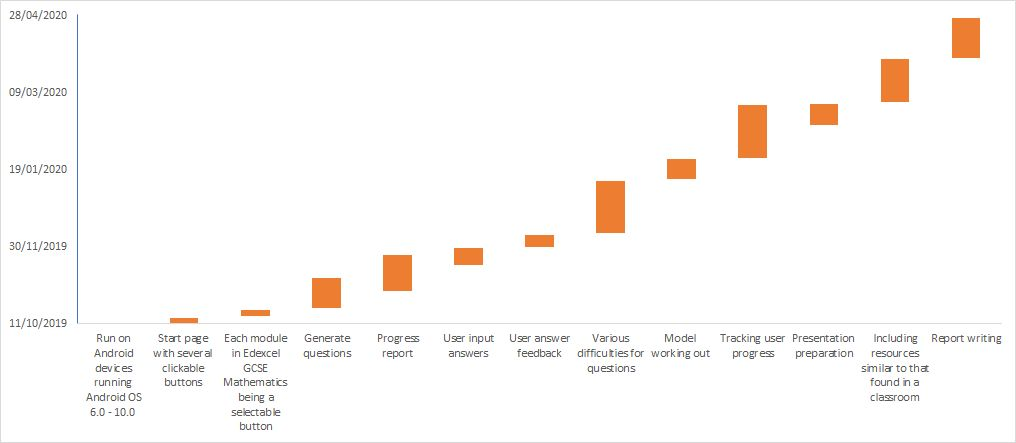
\includegraphics[width=\linewidth]{./data/projectSpecGanttChart.png}}
	\caption{Gantt chart of the schedule produced for the project specification.}
	\label{figure:projectSpecGanttChart}
\end{figure}

This schedule was an optimistic schedule. It assumed all of the requirements would be completed by the end of the project, whereas the project specification's definition of success did not need all requirements to be completed. 

\subsubsection{Progress Report Schedule}

The progress report submitted on 24\textsuperscript{th} November 2019 updated the project specification's schedule. Development was slower than intended throughout the first term of this academic year (October 2019 - December 2019) due to personal reasons, as well as poor project management which has been discussed in detail in the risks section of this report. This updated schedule was created to account for this slow development. The new schedule, referred to from now on as the Christmas schedule, also made the assumption that every requirement would be completed before the final deadline for this project. To mitigate against the slow development conducted through term one of this academic year, the Christmas schedule increased the workload of the project throughout the Christmas period (8\textsuperscript{th} December 2019 - 8\textsuperscript{th} January 2020) and throughout the second academic term of this project. \par

A Gantt chart created for this updated schedule can be viewed below as figure \ref{figure:progressReportGanttChart}. \par

\begin{figure}[H]
	\centering
	\frame{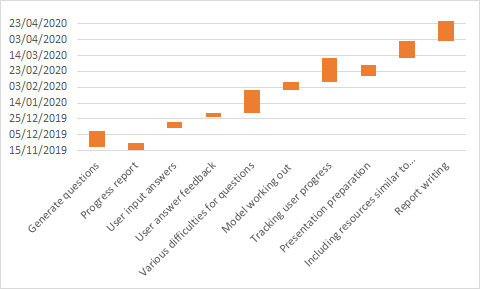
\includegraphics[width=\linewidth]{./data/progressReportGanttChart.png}}
	\caption{Gantt chart of the updated schedule produced for the project specification.}
	\label{figure:progressReportGanttChart}
\end{figure}

Everything before the 24\textsuperscript{th} November 2019 in this Gantt chart is correct as it was completed before this schedule was created. Anything after this date is an estimate, and comparisons for future work should be compared to this. \par

\subsubsection{Schedule Evaluation}

The image displayed below as figure \ref{figure:finalSchedule} shows the final schedule at the end of the project. \par

\begin{figure}[H]
	\centering
	\frame{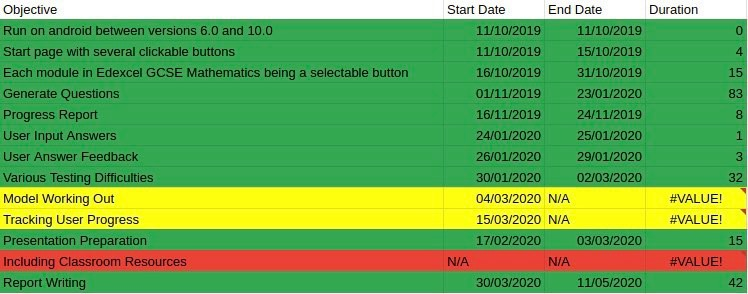
\includegraphics[width=0.9\linewidth]{./data/finalScheduleColour.jpg}}
	\caption{The final schedule created at the end of the project.}
	\label{figure:finalSchedule}
\end{figure} 

This figure displays information about each requirement, as well as some key deliverables produced throughout the project. It shows the start and end dates of the requirements, as well as the duration of each requirement in days. The requirements are colour coded. Requirements with a green background have been fully completed at the end of the project. A yellow background for the requirement represents a started but uncompleted requirement, and a red requirement was not started during the project. \par

This final schedule was behind both the project specification schedule and the progress report schedule. The reasons for this are discussed in the risks section of this report. All of the schedules were optimistic and assumed that all of the requirements would be met. This was different to how the definition of success for this project was defined. Even though the project was behind the optimistic schedules, work was still completed at a satisfactory rate, causing the project to be completed on time. Although, if time was not lost during the first half of development the optimistic schedules could have been met. \par

\subsection{Tools}

This project utilized several tools to aid in the development of this Android application. Two of the main tools used to add value to this project are outlined below.

\subsubsection{Android Studio}

Android Studio[22] was used as an IDE (Integrated Development Environment) throughout development as it comes with many useful features. These features are specifically designed to help with Android app development. Examples of these features are: 

\begin{itemize}
	\item A rendering engine which converts XML into a virtual application display
	\item An android device emulator
\end{itemize}

The rendering engine displays the layout of any XML written in Android Studio. It enables editing the XML directly with any changes made being viewable in the virtual layout in real time, and the ability to edit directly into the rendered layout with a drag and drop feature. This enables quick prototyping for new pages through the use of the drag and drop feature whilst also allowing for a much larger degree of control through the ability to directly edit XML. \par

The Android device emulator can simulate any Android device which it contains files for. Files for new devices can be downloaded through Android Studio, and new devices are being added regularly. This feature enabled quick and efficient testing throughout development. When a new feature was integrated into the application it could be tested on a wide range of devices, ensuring that the application behaved consistently on all Android smartphones and tablets. \par

The Android Studio IDE greatly increased the efficiency of development due to the features stated above. Also, Android Studio being built upon the IntelliJ platform meant that code editing was smooth and intuitive. \par

\subsubsection{Git}

Git was used as the version control software for this project. This enabled access to the project from any device, anywhere, anytime. It also enabled the ability to revert back to an earlier version of the project if something went wrong. This meant that development could take place without fear of failure, as if any changes made broke the project then it could be reverted to the last working state. \par

The repository for this project is available at the link in reference [23]. This repository is public which enables anyone to see the code that would run on their machine. \par

Git automatically logs the time whenever a change is made to the repository. This enabled precise tracking of requirement completion and aided project management. Git commit messages for this project were deliberately helpful and explained changes made to the codebase, so they could be used as logs of when project requirements were completed. The git commit messages for this project can be viewed and give a detailed timeline of when requirements were completed and features were added. This was useful as it gave updates of any changes made to the codebase and is available to anyone who follows the repository as soon as the update is pushed. Git was used to create a timeline of requirement completion for the schedule included in this final report. \par

\subsection{Miscellaneous Project Management}

Weekly meetings were held with the project supervisor to keep key stakeholders up to date with development. Alongside weekly meetings, access was given to the project supervisor and relevant stakeholders to the git repository for this project early in development. \par

A document in the git repository called notes.txt is a file which contains notes created throughout development, such as what was intended to be completed at the beginning of each development session, as well as what was actually completed by the end of the session. A substantial amount of time was spent at the beginning of early development sessions on remembering content added throughout the previous development session, the current state of the code, and what needed to be completed during this development session. Notes.txt cut down the time spent at the beginning of development sessions looking through previous git commits, and so overall this file caused development to be more efficient. \par

\section{Results}
\label{section:results}

This section of the report will evaluate the final application produced for this project and compare it against the requirements and definition of success set out at the beginning of this project. It will also contain the analysis of the project by the author. 

\subsection{Requirements}

The definition of success for this project was defined as such. To be deemed successful, the final product produced by this project will have completed: 

\begin{itemize}
	\item all of the must requirements defined above
	\item at least one of the should requirements defined above
	\item any value of could requirements defined above.
\end{itemize}

The final application satisfies all of the must requirements. This means that the final application can display questions for users to answer, have an input field accepting numerical values, and when an answer is submitted, compare it to the pre-calculated answer and display whether the two answers match. If the two answers do not match, then the pre-calculated answer is displayed for the user to see. \par

One of the three should requirements for this project was completed outright. Requirement 7, which was defined as "having a variety of testing difficulties, ranging from easy to hard for each module" was changed between the progress report and the project presentation. It was changed to "having two separate testing difficulties of foundation and higher for each module". This change was made as the Edexcel GCSE Mathematics specification is split into two difficulty tiers of foundation and higher. The foundation tier of exams range from grades 1-5 and the higher tier exams range from grades 4-9, with the higher tier covering all content in the foundation tier with more complicated content also included to make the higher tier exams more difficult. As the Edexcel tier system already existed using easy, medium, and hard as testing difficulties would only confuse students. Because of this, the decision to switch to Edexcel's difficulty tiers was made. \par

Requirements 8 and 9 were not completed by the end of this project but were in progress. Requirement 8 was defined as "having a way of tracking user progress over a number of days or tests per module", and requirement 9 as "displaying model methods for working out the correct answer for a question where the user inputted an incorrect answer". These requirements have been started and prototypes for each have been created. Model working out has been made for three different questions in the algebra topic. These model working out are displayed when the user submits an incorrect answer. A database was created to store the user's progress, although was never implemented. \par

The could requirement has not been completed. This is because requirements 8 and 9 had to be completed before requirement 10, the could requirement, could have been worked on. As requirements 8 and 9 were incomplete at the end of the project, development for requirement 10 never began. \par

As non-functional requirements are difficult to evaluate, it is a challenging task to determine in absolutes whether these requirements have been met. Any tests conducted with 11 year olds to determine their comprehension of the questions in this application would not have been representative of the population as a whole. Because of this, the method was not used to attempt to assess the completion of the non-functional requirements. Instead, user testing was conducted with colleagues who work with students within the GCSE age range. Their feedback was incorporated into the development process as explained in the testing section of this report. Their feedback on the final application was that the functional requirements have been completed for almost all students who are in the English year 11, and the majority of students in the English year 9. Because of this, these functional requirements have been deemed completed to a satisfactory level for this project. \par

\subsection{Results Overview}

By the definition of success laid out in the project specification this project was successful. All of the must requirements were completed, as well as one of the three should requirements, although the could requirement was left incomplete. \par

Overall, the project produced a proof of concept that the MyMaths homework functionality could be turned into a mobile application which was this project's end goal. The final product from this project could be released on the Google Play store in its current state. Although, if this project were to be extended then the application would not be uploaded to the Google Play store for another two to three months. This extra time would be spent completing the should requirements, and working on the could requirement for content which is examined on the foundational exams. \par

This project could have been improved with better project management throughout the first term of this academic year. The project fell behind early in development as was discussed in the risks section of this report. Improvement was shown in project management as more time progressed. Improvements were made to the authors time management skills, such as dedicating specific time each week to work on the project, as well as calculating the critical path for the features being implemented in this application. These improvements had a large impact on the final product, and counteracted the previous loss of development time from the first academic term. \par

This project was a worthwhile endeavour as it highlights that more work can be completed on mobile GCSE revision applications. Students would benefit from an application endorsed by teachers, which aids in a student's education in GCSE mathematics. This could reducing the barrier of entry for students improving their education to only requiring access to a smartphone, and could increase GCSE grades as most students have regular access to a smartphone, as explained in the introduction of this report. \par

\section{Conclusion}
\label{section:conclusion}

In conclusion, this project was a success. It has produced a proof of concept application which highlights a gap in the GCSE Mathematics revision market. On top of this, the final application produced by this project could be used by GCSE students to aid their revision of GCSE Mathematics, which was the problem that this project aimed to solve. \par

A GCSE Mathematics revision application endorsed by schools will most likely be produced in the future. Throughout the development of this project MyMaths have released an application which is accessible through tablets which currently has a small amount of content accessible, with more being added throughout the coming months[30]. MyMaths have created this tablet application as all of their content before November 2019 was written in the flash multimedia software platform. Adobe announced in July 2017 that it was going to "stop updating and distributing the Flash Player at the end of 2020 and encourages content creators to migrate any existing Flash content to new open formats"[31]. This means that MyMaths is migrating all of their content away from flash, and in doing such are producing an application available on tablets. \par

This project produced software which could be released as an application onto the Google Play store and would be useful for students sitting their GCSE Mathematics examinations from November 2021 onwards. All of the questions in the application have been taken from non-calculator past papers and so no calculator is necessary. Although, the questions could be adapted to include more difficult numbers which would require a calculator. This application could also be updated with new questions after each exam cycle is complete. \par

The development of this application could continue into a commercial product. If the improvements in the future work section of this report are completed then the application would be brought up to paid quality, and so could be released for a small price on the Google Play store. It could also be continuously updated with new features, and the scope of the project increased. \par

\section{Future Work}
\label{section:futureWork}

The final product from this project is not perfect, and could be extended to be released onto the Google play store. This section of the report will outline key changes which would be made to the project if restarted. After, it will explain extensions which would be made to this project if it were to be continued from its current state. \par

\subsection{Project Improvements}

These improvements are changes that would be made to the application if the project was restarted from nothing.

\subsubsection{Question Storage}

Currently, questions are hard coded into the application which has several disadvantages. One of the disadvantages is that any changes made to a question would only be available to users through downloading application updates. This delays question changes getting to users and would cause lots of small app updates. Another disadvantage to hard coding questions is that users cannot add their questions to the pool used within the application. This is because users do not have access to, and cannot change, the source code of the application. \par

There are two methods which could be implemented to store questions within the application, both with benefits and drawbacks and both would require a change in the question display logic. \par

The first method of question storage would be to write the questions to a JSON file stored locally on the system. This would allow the manipulation of questions (inserting questions, updating questions, deleting questions, etc) locally. This would enable users to add questions just by appending an element to the JSON file. The small update to the current question logic would be to change from iterating through an Array list storing Java string types to iterating through the data in a JSON object. The data would not be rewritten each update. This is because a second JSON file would be added which contains the user added questions which would not be rewritten when there was an update overwriting the JSON file containing the developer created questions. \par

The second method of question storage would be to insert elements into a database which would have the benefit of being persistent local storage. SQLite is built into Android and so it would be easy to implement. It would, however, require a complete rewriting of the question logic. This is due to it iterating through Array lists. Instead, the question logic would need to query the database, fetch some relevant data, find a way of displaying that data, and generate the random numbers necessary as per the requirements for this project. \par

If this project were to be restarted then the method for implementing question storage would depend on the amount of question data that is required to be stored. For smaller amounts of question data the JSON file method would be used. This is because iterating through a JSON file until the right question is found would not add too much time onto question generation. The convenience of creating a working implementation of the JSON storage method would be too great to justify using the database method. Although, when the JSON file gets large, iterating through questions until one specific question is found would be time consuming. In this situation a database would be used. SQLite would be much faster at locating a specific row in the database than iterating through the JSON file. \par

\subsubsection{Accessibility Improvements}

If this project were to be restarted then accessibility issues would be much higher on the list of priorities than it was. Questions could be played in audio form to aid those users who are visually impaired. Audio files could be saved to the users device and played to explain any questions that could be generated through normal use of the application. Also, when an answer is inputted the value could be spoken aloud, or in the case of a multiple choice question the selected answer could be read aloud. This would enable users which have some form of visual impairment to be able to use the application. \par

There could also be a setting which increases the font size of all text within the application, and would also increase image size. This would aid users with visual impairments, and would be built into the application from the first version. Although, there is an option to increase the font size from within the Android operating system settings. \par

\subsubsection{Content Grouping}

Content within the application could be grouped into the appropriate age ranges as well as by module. This would aid younger students, those ranging from academic years 7 to 9, to utilise this application for revision. This would increase the usage of the application, and aid more students in their understanding of GCSE Mathematics. \par

Currently, any students between the ages of 11 and 14 who wish to use the application could get questions about content that they have not yet covered in the classroom. This is counterproductive to the aims of this application, as students would become frustrated that they cannot answer a given question, and they are less likely to continue using the application. Instead, with content grouped into appropriate academic years, as well as modules, students can be certain that the questions they are attempting are appropriate to their situation. \par

\subsubsection{Trello}

If the project was restarted then some decisions would be changed to improve productivity. Development would be started later to allow for effective preparation of a project this size. Certain PMBOK processes would have been followed in the planning phase of this project. For example, developing a schedule should have consisted of defining activities to be completed which produce deliverables, sequence the activities depending on their dependencies, estimate how long each activity would take, and then creating the timeline for the project. Instead, this project estimated the amount of time each requirement was expected to take, and estimating the completion of a task is harder than estimating the completion of a deliverable. \par

Deliverables for this project would be made from each requirement, which would make estimating the time to complete this project easier. Once the deliverables for this project were created, they could then be entered into a Trello[29] board which would have allowed for more effective management. Trello is an organisational tool, and was used by the author as a to-do list whilst writing this report. Boards can be created which contain deliverables to remind team members which items still need to be completed. Figure \ref{figure:trelloBoard} shows the Trello board for this report: 

\begin{figure}[H]
	\centering
	\frame{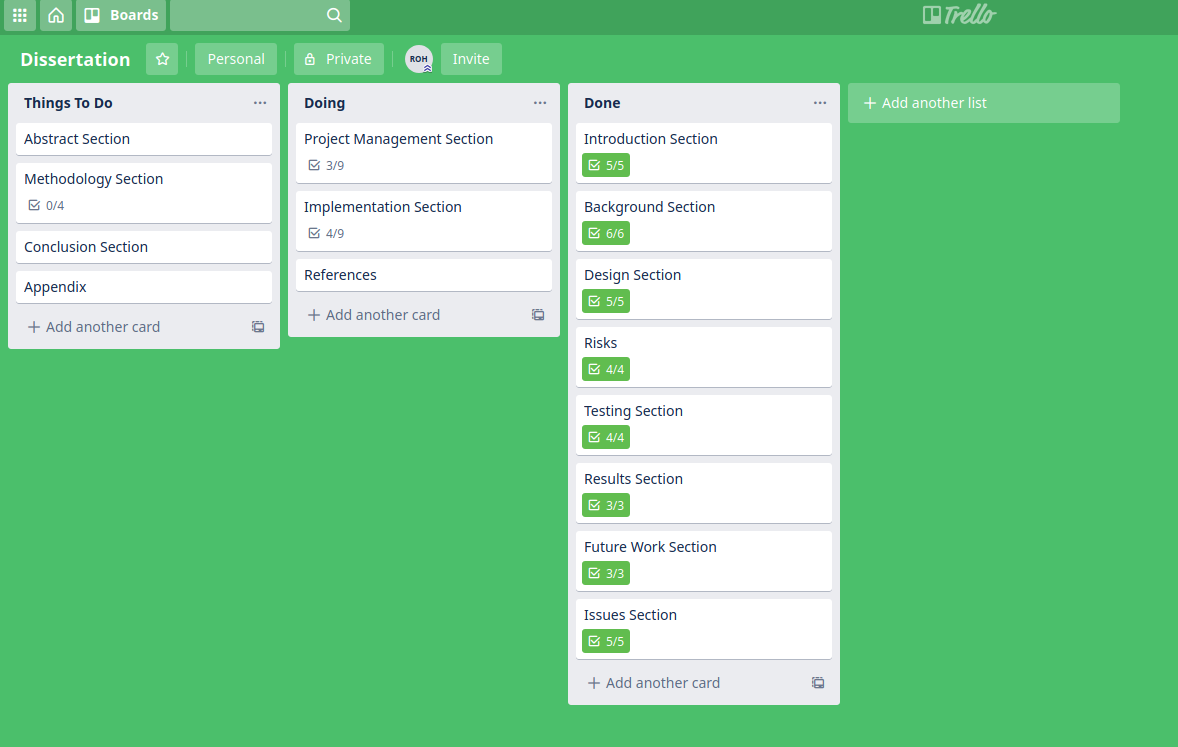
\includegraphics[width=0.9\linewidth]{./data/trelloBoard.png}}
	\caption{Trello board used as a to-do list for this report.}
	\label{figure:trelloBoard}
\end{figure}

The figure above displays a to-do list for this report at the time of writing this section. Using Trello as a to-do list for the deliverables of this report greatly increased productivity. This was due to increased preparation time for the final report, as opposed to the development cycle. Also, the Kanban software development methodology was used throughout the report writing process which increased productivity throughout this time. \par

If this project was restarted from scratch then Trello would be used, alongside the Kanban project management methodology to improve efficiency and eliminate waste throughout this project. \par

\subsection{Project Extensions}

Project extensions are features which would be added to the application if this project continues from its current state. 

\subsubsection{Currently Uncompleted Requirements}

If this project continues the first thing that will be completed are the three uncompleted requirements. These are requirement 8, 9, and 10. This will mean that the application will track users recent feedback, display model answers when the user gets an answer incorrect, and there will be some kind of classroom like learning resource. \par

These requirements were in the original scope of the project but due running out of time they were incomplete at the end of the project. This is why they would be completed first if extra time was added onto this project, as requirements 8 and 9 are already in the prototype phase and could be fully implemented into the application given an extra month. 

\subsubsection{User Validation}

User validation would be a key feature which would be added to the application. Two types of user accounts would be created, those available for students and those available for teachers. Student accounts will be able to attempt any question from any module in any year group. They would have full access to all testing and learning content at any time. Teachers will have the ability to create classes which will contain a group of students from the same academic year. \par

User validation was outside the scope of the project as there are many potential legal issues with storing user data. This application would have to register under the data protection act and ensure that all data collection is compliant under the new GDPR law as this application would be only used within the United Kingdom. It was deemed that the potential legal issues which come with storing user data was not worth the risk for a project of this scope. This is why if the scope was increased and time was added onto this project then these potential legal issues would be solved. \par

A user would need to have the ability to register an account with an email to utilise certain features present within the application. A single sign on (SSO) feature can also be added to allow users to sign in with other popular accounts such as Facebook and Google. This would shift the burden of sign on security to the validating third party, although would not be practical for all cases. A user may not have a third party account and so there would need to be the ability for a user to register an account with their email as well. \par

\subsubsection{User Added Questions}

A feature which would be useful is users being able to add their own questions to the question pool of this application. This was deemed outside of the scope for the current project as this is not a feature available in any of the major GCSE Mathematics revision applications. This feature would only be added after the question storage method is changed, as currently there is no way to automate adding a question into the question pool due to how questions are stored. \par

This feature would only be available for user initiated testing and would not be analysed by the statistical tools which would be built into the application as requirement 8. This is to prevent students from abusing the question adding process. A student could add questions which have a single, simple answer, or are much simpler than other questions in the same skill level. If the questions were analysed then a student could abuse the question adding mechanism so that they get 100\% in a homework or revision set. \par

This feature would be implemented by adding an activity which would allow the user to input details for a new question. Users would utilise radio buttons to select the module and submodule for the specific question, as well as the year if that feature had been implemented. There would be a text box where users could type out the question text, and a specific set of characters would be used to represent variables which the application has to generate. This set of characters would then be found using regular expressions. \par

\subsubsection{MyMaths Homework Feature}

If the scope of this project was increase then a homework feature, similar to that of MyMaths homework feature, could be implemented. This would allow teachers to set their classes revision tests to be completed by a given date. Students would require over a certain percentage score in these tests to pass the homework, but they have no attempt limit. The students would then be notified of the homework via push notifications, as well as something visual within the application, preferably on the homepage so students do not miss it. \par

Students could then attempt the specific homework with their highest score being sent to the teacher to analyse. If a student achieves a score below the passing grade for that homework, then they could reattempt the homework, or look at some revision materials for that specific topic. These homework questions would be separate from the user added questions, for reasons of integrity discussed above. \par

Teachers could also be provided with the ability to select specific questions for a topic, and change the appearance probability. This would grant teachers the flexibility to customise a homework specifically for their class. \par

\section{Legal, Social, Ethical, and Environmental Issues}
\label{section:issues}

This project did not face many legal, social, ethical, or environmental issues throughout development. There were no environmental or social issues faced for this project. There were limited legal and ethical issues which will be discussed in this section of the report under their respective subheadings. 

\subsection{Legal Issues}

There was one legal issue faced throughout this project. This issue was related to the tools which were used. As the final source code was not wholly developed by the development team there may have been some legal issues regarding licensing. Some of the code was generated through the tools used to aid this project, for example any code pre-generated through the Android Studio IDE which was included in the final source code could create legal issues due to copyright laws. \par

This is why the licensing for all of the tools used is linked below as a reference, and relevant sections are quoted to ensure that there are no legal issues caused by this project. \par

\subsubsection{Android Studio}

Android Studio is built on top of the IntelliJ platform. It shares the same license as IntelliJ, as is shown in this comment on a blog post by the creator of IntelliJ Dmitry Jemerov (Yole in the blog post) [24]. The IntelliJ IDEA[25] (the IntelliJ IDE) is licensed under two licenses, but as is explained in the blog post, the licensed version of IntelliJ IDEA that is used as the basis of Android Studio has the Apache 2 license. The relevant sections of the Apache 2 license are as follows: "You may reproduce and distribute copies of the Work or Derivative Works thereof in any medium, with or without modifications, and in Source or Object form"[26]. This allows for the use of the IntelliJ and Android Studio IDEs for commercial and independent development which this project falls under, and so there are no legal issues with using Android Studio as the IDE for this project. \par

\subsubsection{Git}

The majority of git is released under the GNU public license [27] which enables copying, modifying, or distributing git under any circumstances. The relevant sections of the GNU licence (from the preamble): "By contrast, the GNU General Public License is intended to guarantee your freedom to share and change free software--to make sure the software is free for all its users.". This enables free use of git for this project. \par

Small sections of git are not licensed under the GNU public license, but under the GPL (GNU Lesser Public License) [28]. Relevant sections from the GPL preamble: "By contrast, the GNU General Public Licenses are intended to guarantee your freedom to share and change free software--to make sure the software is free for all its users". This section of the license refers to the GNU General Public Licenses, which the GPL is included as a part of. This enables the free use of git for this project. \par

As these are the only two external tools used throughout this project, and the only tools which could have impact on the source code of this project, then there are no legal issues caused by this project. Any other materials were produced by the author specifically for this project, and so there are no legal problems with using these materials. \par

\subsection{Ethical Issues}

This project contains one ethical issue, which is to do with the testing of the final product. Testing was conducted on colleagues who gave verbal consent to participate in the testing of the application. This testing method makes this project one which does not require ethical review under the departmental guidelines found here [29]. "Student projects with primarily an educational purpose, for example asking peers or family members to test software as part of your course. Such projects should not include any form of deception or coercion or involve vulnerable groups (e.g. schoolchildren)." As testing was not conducted on vulnerable groups for this project, as user testing was conducted on colleagues over the age of 18, this project has no ethical issues. 

\section{References}
\label{section:references}

[1] - https://www.gov.uk/government/speeches/reformed-gcses-in-english-and-mathematics (Accessed 29\textsuperscript{th} March 2020) \par

[2] - https://qualifications.pearson.com/en/qualifications/edexcel-gcses/mathematics-2015.html (Accessed 29\textsuperscript{th} March 2020) \par

[3] - https://www.pewresearch.org/internet/2018/05/31/teens-social-media-technology-2018/ (Accessed 30\textsuperscript{th} March 2020) \par

[4] - https://www.comscore.com/Insights/Presentations-and-Whitepapers/2017/2017-US-Cross-Platform-Future-in-Focus (Accessed 30\textsuperscript{th} March 2020) \par

[5] - https://gs.statcounter.com/os-market-share/mobile/worldwide (Accessed 30\textsuperscript{th} March 2020) \par

[6] - https://qualifications.pearson.com/content/dam/pdf/GCSE/mathematics/2015/specification-and-sample-assesment/gcse-maths-2015-specification.pdf (Accessed: 6 October 2019) \par

[7] - https://www.mymaths.co.uk/ (Accessed 22\textsuperscript{th} March 2020) \par

[8] - https://www.mymaths.co.uk/help.html (Accessed 22\textsuperscript{th} March 2020) \par

[9] - https://www.khanacademy.org/ (Accessed 22\textsuperscript{th} March 2020) \par

[10] - https://www.khanacademy.org/math/trigonometry/trig-with-general-triangles/law-of-sines/v/law-of-sines (Accessed 22\textsuperscript{th} March 2020) \par

[11] - https://apps.apple.com/gb/app/khan-academy/id469863705 (Accessed 22\textsuperscript{th} March 2020) \par

[12] - https://play.google.com/store/apps/details?id=org.khanacademy.android (Accessed 22\textsuperscript{th} March 2020) \par

[13] - https://mathswatch.co.uk/ (Accessed 25\textsuperscript{th} March 2020) \par

[14] - http://www.mathswatch.co.uk/subscription/4594745491 (Accessed 25\textsuperscript{th} March 2020) \par

[15] - http://coolt.ch/notizen/wp-content/uploads/2016/02/Head-First-Android-Development-2015.pdf (Accessed 31\textsuperscript{th} March 2020) \par

[16] - https://developer.android.com/docs (Accessed 31\textsuperscript{th} March 2020) \par

[17] - https://github.com/AlphaMustang (Accessed 31\textsuperscript{th} March 2020) \par

[18] - https://trello.com/ (Accessed 8\textsuperscript{th} March 2020) \par

[19] - https://developer.android.com/guide/components/activities/intro-activities (Accessed 28\textsuperscript{th} March 2020) \par

[20] - https://developer.android.com/guide/components/fragments (Accessed 28\textsuperscript{th} March 2020) \par

[21] - https://developer.android.com/studio/run/emulator (Accessed 26\textsuperscript{th} March 2020) \par

[22] - https://developer.android.com/studio (Accessed 17\textsuperscript{th} April 2020) \par

[23] - https://github.com/AlphaMustang/thirdYearProject (Accessed 28\textsuperscript{th} March 2020) \par

[24] - https://blog.jetbrains.com/idea/2013/05/intellij-idea-and-android-studio-faq/\#comment-4939 (Accessed 29\textsuperscript{th} March 2020) \par

[25] - https://www.jetbrains.com/idea/features/ (Accessed 29\textsuperscript{th} March 2020) \par

[26] - https://www.apache.org/licenses/LICENSE-2.0 (Accessed 29\textsuperscript{th} March 2020) \par

[27] - https://github.com/git/git/blob/master/COPYING (Accessed 22\textsuperscript{th} March 2020) \par

[28] - https://github.com/git/git/blob/master/LGPL-2.1 (Accessed 22\textsuperscript{th} March 2020) 2020) \par

[29] - https://warwick.ac.uk/fac/sci/dcs/teaching/ethics (Accessed 22\textsuperscript{th} March 2020) \par

[30] - https://support.mymaths.co.uk/technical-support/what-mymaths-content-has-been-updated/ (Accessed 16\textsuperscript{th} April 2020) \par

[31] - https://theblog.adobe.com/adobe-flash-update/ (Accessed 16\textsuperscript{th} April 2020) \par

[32] - Head first android development pg 312

[33] - https://www.agilealliance.org/glossary/poker/ (Accessed 20\textsuperscript{th} April 2020)

\end{document}